%%%%%%%%%%%%%%%%%%%%%%%%%%%%%%%%%%%%%%%%%
% Diaz Essay
% LaTeX Template
% Version 2.0 (13/1/19)
%
% This template originates from:
% http://www.LaTeXTemplates.com
%
% Authors:
% Vel (vel@LaTeXTemplates.com)
% Nicolas Diaz (nsdiaz@uc.cl)
%
% License:
% CC BY-NC-SA 3.0 (http://creativecommons.org/licenses/by-nc-sa/3.0/)
%
%%%%%%%%%%%%%%%%%%%%%%%%%%%%%%%%%%%%%%%%%

%----------------------------------------------------------------------------------------
%	PACKAGES
%----------------------------------------------------------------------------------------

\documentclass[draft, 11pt]{diazessay} % Font size (can be 10pt, 11pt or 12pt)

\usepackage[
    type={CC},
    modifier={by-nc-sa},
    version={3.0},
]{doclicense}

%----------------------------------------------------------------------------------------
%	Link Colors
%----------------------------------------------------------------------------------------
\usepackage{hyperref}
\usepackage[table]{xcolor}
\usepackage[normalem]{ulem}
\hypersetup{colorlinks,urlcolor=blue}
%% or
% \hypersetup{colorlinks=false,pdfborder=000}
% hack into hyperref
\makeatletter
\DeclareUrlCommand\ULurl@@{%
  \def\UrlFont{\ttfamily\color{blue}}%
  \def\UrlLeft{\uline\bgroup}%
  \def\UrlRight{\egroup}}
\def\ULurl@#1{\hyper@linkurl{\ULurl@@{#1}}{#1}}
\DeclareRobustCommand*\ULurl{\hyper@normalise\ULurl@}
\makeatother

\usepackage[numbers]{natbib} % bibliography style

\usepackage{amsmath, amssymb, latexsym}
\usepackage{minted} % code formatting

 % 3D plots and tikz images
\usepackage{tikz}
\usepackage{tikz-3dplot} 
\usetikzlibrary{shapes,arrows,chains,positioning,shapes.geometric,arrows.meta,backgrounds,fit, shapes}

\usepackage{forest} % trees
\usepackage{float}

%----------------------------------------------------------------------------------------
%	Shape Styles for Images
%----------------------------------------------------------------------------------------
% Define block styles
\tikzstyle{decision} = [diamond, draw, fill=blue!20, 
    text width=4.5em, text badly centered, node distance=3cm, inner sep=0pt]
\tikzstyle{block} = [rectangle, draw, fill=blue!20, 
    text width=5em, text centered, rounded corners, minimum height=4em]
\tikzstyle{line} = [draw, -latex']
\tikzstyle{cloud} = [draw, ellipse,fill=red!20, node distance=3cm,
    minimum height=2em]
    \tikzstyle{mybox} = [draw=red, fill=blue!20, very thick,
    rectangle, rounded corners, inner sep=10pt, inner ysep=20pt]
\tikzstyle{fancytitle} =[fill=red, text=white]
%----------------------------------------------------------------------------------------
%	TOC
%----------------------------------------------------------------------------------------
\setcounter{secnumdepth}{4} % how many sectioning levels to assign numbers to
\setcounter{tocdepth}{4}    % how many sectioning levels to show in ToC

%----------------------------------------------------------------------------------------
%	CAPTIONS
%----------------------------------------------------------------------------------------

\usepackage{subcaption}
\DeclareCaptionFormat{custom}
{%
    \textbf{#1#2}\textit{\small #3}
}
\captionsetup{format=custom}


%----------------------------------------------------------------------------------------
%	TITLE SECTION
%----------------------------------------------------------------------------------------
\begin{document}

\thispagestyle{empty}

\begin{tikzpicture}[remember picture, overlay]
\node[anchor=north west, inner sep=0pt] at (current page.north west) {\includegraphics[width=\paperwidth, height=.5\paperheight]{figures/kandinsky.jpg}};
\node[below=1cm of current page.center, align=center, font=\Huge\bfseries] {What are embeddings};
\node[below=2cm of current page.center, align=center, font=\Large\bfseries] {Vicki Boykis};
\node[below=3cm of current page.center, align=center, font=\large\bfseries] {\today};
\end{tikzpicture}

\begin{tikzpicture}[remember picture, overlay]

  \draw[line width=2pt] (current page.south west) ++(0,2cm) -- ++(\paperwidth,0);
\end{tikzpicture}

\newpage

%----------------------------------------------------------------------------------------
%	ABSTRACT AND META
%----------------------------------------------------------------------------------------

\begin{abstract}
Over the past decade, embeddings, vector representations of textual elements, have become a foundational data structure in machine learning architectures. Although reducing dimensionality as a concept has always been important in machine learning systems to decrease computational and storage complexity through methods like TF-IDF, PCA, and one-hot encoding, compression has become even more important in the modern explosion of multimodal representations of data that comes from application log files, images, video, and audio. 

Google's \href{https://arxiv.org/abs/1301.3781}{Word2Vec paper} made embeddings, an intermediate output of a neural network model, more accessible for natural language projects, and consequently, for other downstream machine learning work. The subsequent rise of the \href{https://arxiv.org/abs/1706.03762}{Transformer architecture} and transfer learning enabled the growth of embeddings as a foundational structure. 

The goal of this paper is to provide both a broad and deep dive into what embeddings are, their history, and current usage patterns both for any stakeholders working with embeddings in an industrial context, and for the machine learning practitioner considering them for their project. 

\end{abstract}

\section*{About the Author}

Vicki Boykis is a machine learning engineer. You can find her main website at \href{https://www.vickiboykis.com}{vickiboykis.com} and Viberary, her semantic search side project at \href{https://www.viberary.pizza}{viberary.pizza}. Send all typos, comments, and questions to \href{mailto:vickiboykis@gmail.com}{vickiboykis@gmail.com}

%----------------------------------------------------------------------------------------
%	CREATIVE COMMONS LICENSE
%----------------------------------------------------------------------------------------

\section*{Acknowledgements}
Lorem ipsum dolor sit amet, consectetur adipiscing elit, sed do eiusmod tempor incididunt ut labore et dolore magna aliqua. Ut enim ad minim veniam, quis nostrud exercitation ullamco laboris nisi ut aliquip ex ea commodo consequat. Duis aute irure dolor in reprehenderit in voluptate velit esse cillum dolore eu fugiat nulla pariatur. Excepteur sint occaecat cupidatat non proident, sunt in culpa qui officia deserunt mollit anim id est laborum.

Lorem ipsum dolor sit amet, consectetur adipiscing elit, sed do eiusmod tempor incididunt ut labore et dolore magna aliqua. Ut enim ad minim veniam, quis nostrud exercitation ullamco laboris nisi ut aliquip ex ea commodo consequat. Duis aute irure dolor in reprehenderit in voluptate velit esse cillum dolore eu fugiat nulla pariatur. Excepteur sint occaecat cupidatat non proident, sunt in culpa qui officia deserunt mollit anim id est laborum.


\section*{License}
\doclicenseThis
\newpage

%----------------------------------------------------------------------------------------
%	TOC
%----------------------------------------------------------------------------------------
\tableofcontents
\newpage

%----------------------------------------------------------------------------------------
%	ESSAY BODY
%----------------------------------------------------------------------------------------

\section{Introduction}

Machine learning has grown rapidly in adoption across many modern web applications. With its ascent, embeddings are quickly becoming a critical idiom in building machine learning systems that need to process large quantities of unstructured data like text, video, and audio. This means that both engineers who build these systems and technical leadership that signs off on them need to understand them.  But in my deep-dive into the embeddings reference material, I found that there are two types of resources: very deeply technical academic papers, for people who are already NLP experts, and surface-level marketing spam blurbs for people looking to buy embeddings-based tech, and that neither of these take each other into account.  I wanted a resource that was technical enough to be useful enough to ML practitioners, but one that also put embeddings in their business context as they become more often used in ML architecture stacks. This is, hopefully, that text. 

As Nick Seaver \citep{seaver2022computing} writes in "Computing Taste", his study of music recommendation systems and companies,

\begin{quote}
"[Most] technical systems are best understood as sociotechnical systems- as hybrid agglomerations of elements that are both human and machine. While popular and academic critics might pit humans against algorithms, these "algorithms" were full of people making decisions, changing things around, and responding to a never-ending stream of small and large crises."
\end{quote}

Let's examine embeddings from three critical perspectives: business context, machine learning theory, and engineering implementation. In writing this text, I strove to balance the need to have precise technical and mathematical definitions for concepts and my desire to stay away from explanations that make people's eyes glaze over. I've defined all technical jargon when it appears to build context. Regardless, it would be helpful for the reader to have some familiarity with programming and machine learning for the sections where I go in-depth. But, ultimately the goal is to educate anyone who is willing to sit through this, regardless of level of technical understanding. 


\section{Recommendations as a business problem}

We'll start at the highest level. Let's motivate this paper with an example business case that should make it easier to grasp what are very abstract and technical concepts. We run a social media app, \textbf{Flutter}, the premier social network for all things with wings. Flutter is an app where users can post short snippets of text, videos, images, and sounds, to let other birds, insects and bats in the area know what’s up. Its business model is based on targeted advertising, and its app architecture includes a home feed made up of small pieces of multimedia content called “flits”, which can be either text, videos, or photos. 

Flits are either organically sourced from other birds the user follows, as well as personalized, recommended flits so that the user engages further with the platform. When we architect Flutter’s home timeline  it might have a stream of recommendations from different locations. The primary feed might be Flits from birds we follow. It will definitely have ad injections since it's an ad-sponsored platform. The rest is up to the implementation of the recommendations team.

\begin{figure}[!ht]
\centering
\includegraphics[width=.4\textwidth]{figures/timeline.png}
\caption{A generic content timeline in a social feed with a blend of organic followed content, advertising, and recommendations.}
\end{figure}

From a business product perspective, the objective is to offer Flutter’s users content that is relevant, interesting, and novel so they continue to use the platform. In subscription-based platforms like Netflix, this is a clear business objective that's tied directly to the bottom line, as outlined in this paper \citep{steck2021deep}  about Netflix's recsys in 2015: 

\begin{quote}

The main task of our recommender system at Netflix is to help our members discover content that they will watch and enjoy to maximize their long-term satisfaction. This is a challenging problem for many reasons, including that every person is unique, has a multitude of interests that can vary in different contexts, and need a recommender system most when they are not sure what they want to watch. Doing this well means that each member gets a unique experience that allows them to get the most out of Netflix. As a monthly subscription service, member satisfaction is tightly coupled to a person’s likelihood to retain with our service, which directly impacts our revenue.
\end{quote}

In ad-based services, the line between retention and revenue is a bit murkier, and we have often what's known as a multi-stakeholder problem, where the actual optimized function is a balance between meeting the needs of the user and meeting the needs of the advertiser\citep{zheng2017multi}.  In real life, this can often result in a process of enshittifcation\citep{doctorow_2023} of the platform that leads to a race to the bottom. So, when we create Flutter, we have to be very careful to balance these concerns, and we'll also assume for the sake of simplification that Flutter is a Good service that loves us as users and wants us to be happy (as long as we don't have any content that deters advertisers.)

So, how and why might we use embeddings in machine learning workflows in Flutter to optimize this feed so that users are recommended Flits from users they follow but may have missed, or users they don’t follow at all?  Most importantly, how do we show users Flits that are interesting to them personally, knowing that personalized content is more relevant and generally gets higher rates of engagement\citep{jannach2010recommender}  on online platforms than non-personalized forms of recommendation (for more, see  \href{http://www.recommenderbook.net/media/Recommender_Systems_An_Introduction_Chapter08_Case_study.pdf}{this case study} on personalized recommendations in mobile games)? 

What is of more interest than embeddings themselves is the process of generating them and how they relate to one another to give us ways to map semantically and contextually similar items. As such, they’re an important concept to understand we're working with any domain data where there is an extremely large corpus of items that you need to either compare or rank (books, clothes, images, songs, posts, videos, and for us, Flits).


\subsection{Building a web app}
In many cases, we can approach engineering solutions without involving machine learning. In fact, we should definitely start without it\citep{zinkevich2017rules} because it adds a tremendous amount of complexity to our working application\citep{sculley2014machine}. 

\begin{figure}[!ht]
\centering
\includegraphics[width=\textwidth]{figures/solutions.png}
\caption{Approaches for solving an engineering problem }
\end{figure}

Most of the apps we use today --- Spotify, Gmail, Reddit, Slack, and, now Flutter ---   all follow the same basic software engineering design patterns. They are all apps available on web and mobile clients. They all have a front-end where the user interacts with the various features\footnote{Features have many different definitions in the case of machine learning and engineering. In this specific case, we mean collections of code that make up some front-end element, such as a button or a panel of recommendations.} of the applications, an API that connects the front-end to back-end elements, and a database that processes data and remembers state. This is known as \textbf{model-view-controller} pattern \citep{fowler2012patterns}, or in common industry, a \textbf{CRUD} app, named for the basic operations that its API allows to manage application state: create, read, update, and delete. 
 
\begin{figure}[H]
\centering
\includegraphics[width=.9\textwidth]{figures/web_service.png}
\caption{Typical CRUD web app architecture}
\end{figure}

When we think of structural components in the architectures of these applications, we might think first in terms of features. In an application like Slack, for example, we have the ability to post and read messages, manage notifications, and add custom emojis. Each of these can be seen as an application feature. In order to create features, we have to combine common elements like databases, caches, and web services. All of this happens as the client talks to the API, which talks to the database to process data. At a more granular, program-specific level, we might think of foundational data structures like arrays or hash maps, and lower still,we might think about memory management and network calls. These are all foundational elements of modern programming. 

At the feature level, though, we see that it not only includes the typical CRUD operations, such as the ability to post and read Slack messages, but also elements that are more than pure database operations: they involve machine learning components. Some features such as \href{https://slack.engineering/personalized-channel-recommendations-in-slack/}{personalized channel suggestions}, \href{https://slack.engineering/search-at-slack/}{returning relevant results through search queries}, and \href{https://slack.engineering/email-classification/}{predicting Slack connection invites} require machine learning.

In the case of Flutter, also,machine learning forms a business-critical function part of Flutter's product offering. From a business product perspective, the objective is to offer Flutter’s users content that is relevant\footnote{The specific definition of a relevant item in the recommendations space varies, but generally it means an item that is of interest to the user}, interesting, and novel so they continue to use the platform. 

\begin{figure}[!ht]
\centering
\includegraphics[width=\textwidth]{figures/web_service_ml.png}
\caption{CRUD app with ML}
\end{figure}

\subsection{Machine learning in the context of an engineering system}
Machine learning platforms sit within the backend of applications, typically integrated into production workflows, but processing data much differently, and use the application's data to generate machine learning models that act upon and feed data back into the application, to the user. 

In order to understand how embeddings would help here, it first  makes sense to understand how machine learning works at Flutter, or any given company, as a whole. In a typical consumer-facing social company, the user-facing app  is made up of features written in code. Features are a broad concept, but generally something that changes the functionality of the app and can include the “home timeline” or “feed of recommendations” or “button that allows us to mute crows” or “ability to post images”. 

To add a new feature,  we add logic, which acts on data in the app to develop our new feature and add that back into the application. The logic may not always be entirely straightforward, but the process itself is. When we think of the typical software development lifecycle, it looks like this.

\begin{figure}[!ht]
\centering
\includegraphics[width=.75\textwidth]{figures/app_flow.png}
\caption{A typical application development lifecycle flow }
\end{figure}

For applications powered by machine learning, though, we need to start not with an action item, i.e. code that triggers a button toggle, but input data that we use to build a model that will suggest pieces of content. This requires thinking about application development slightly differently, and when we write an application that includes machine learning models as input, however, we’re inverting the traditional app flow. What we have instead, is data + our desired outcome. The data is combined into a model, and it is this model which instead generates our business logic. 

\begin{figure}[!ht]
\centering
\includegraphics[width=.75\textwidth]{figures/ml_flow.png}
\caption{ML Development lifecycle}
\end{figure}

In short, the difference between programming and machine learning development is that we are generating not answers through action, but rules through data.

\begin{figure}[H]
\centering
\begin{tikzpicture}[node distance=4cm]

% Input nodes
\node (rules) at (-2,0) {Rules};
\node (data1) at (-2,-4) {Data};

% Box node
\node[draw,align=center,minimum width=2cm,minimum height=2cm] (prog)  [block]  at (2, -2) {Programming};

% Output node
\node (ans1) at (6, -2) {Answers};

% Arrows
\draw[->, thick] (rules) -- (prog);
\draw[->, thick] (data1) -- (prog);
\draw[->, thick] (prog) -- (ans1);

% Second chart
% Input nodes
\node (data2) at (-2,-8) {Data};
\node (ans2) at (-2,-12) {Answers};

% Box node
\node[draw,align=center,minimum width=2cm,minimum height=2cm] (ml)  [block]  at (2, -10) {Machine\\Learning};

% Output node
\node (ans3) at (6, -10) {Rules};

% Arrows
\draw[->, thick] (data2) -- (ml);
\draw[->, thick] (ans2) -- (ml);
\draw[->, thick] (ml) -- (ans3);

% Centering line
\draw[dashed, thick] (-4, -6) -- (8, -6);

\end{tikzpicture}
\caption{Generating answers via machine learning. The top chart shows a classical programming approach with rules and data as inputs, while the bottom chart shows a machine learning approach with data and and answers as inputs. \citep{chollet2021deep}}
\end{figure}

\subsection{Building a web app with machine learning}
Let's dive deeper into the machine learning stack. 

\begin{figure}[!ht]
\centering
\includegraphics[width=.75\textwidth]{figures/ml_system.png}
\caption{CRUD app with ML}
\end{figure}

The four critical components of a machine learning component are\footnote{There are infinitely many layers of horror of ML systems\citep{kreuzberger2022machine}. These are still the core components. }:

\begin{itemize}
  \item \textbf{Data ingest} - processing data from a database or streaming from a production application for use in modeling
  \item \textbf{Feature selection} - The process of examining the data and cleaning it to pick features\footnote{in this case, we mean features as attributes of any given element that we use as inputs into machine learning. Examples of features are: user name, geographic location, how many times they've clicked on a button for the past 5 days, revenue, and many more} for machine learning. This piece always takes the longest in any given machine learning system
  \item \textbf{Building the model} - We select the features that are important and train our model, iterating on different performance metrics over and over again.
  \item \textbf{Serving the model} - Now that we have a model we like, we serve it to production, where it hits a web service, potentially cache, and our API where it then propagates to the front-end for the user to consume as part of our web app
\end{itemize}

\subsection{Building a web app with a recommender system}

Let's dig into this one layer further to understanding, from an engineering perspective, what a recommendation system looks like. 

\begin{figure}[!ht]
\centering
\includegraphics[width=\textwidth]{figures/recsys.png}
\caption{Recommender systems as an ML problem}
\end{figure}

First, we have the data that we ingest from the production application. This data goes into the the initial piece, which hosts our first-pass model generating \textbf{candidate recommendations}. This is what BERT, Word2Vec, tf-idf and all the other approaches we cover in this paper entail. We then \textbf{filter}, down from potentially millions of generated candidate pieces of media, text, etc, to hundreds.For example, in the case of Flits, maybe we don't want Flits that are NSFW, or don't match particular topics.  Finally, we need a way to order the filtered list of recommendations based on what we think the user will perfer the most, so the next stage is \textbf{ranking}, and then we serve them out in the timeline or the ML product interface we're working with. 

What is the input data that we use as features in our machine learning system? Just as database have become lingua franca in building backend infrastructure to perform data lookups, \textbf{embeddings}, a matrix-based data structure that learns and creates semantic connections between all of the elements of machine learning input datasets, have become similar building blocks in the creation of many modern search and recommendation product architectures.We can think of embeddings as a type of \textbf{feature} that we use as input into the feature engineering step of our models.  

For example, they make up a significant part of Spotify's item recommendation systems \citep{hansen2020contextual} in features like Radio which seed a playlist of your favorite songs and songs similar to those based on a set of embeddings created from song metadata, YouTube video recommendations of what to watch \citep{covington2016deep} , and Pinterest's visual search \citep{jing2015visual}. Even if they are not explicitly presented to the user, embeddings are used internally at places like Netflix to make content decisions around which shows to develop based on user preference popularity. 

\begin{figure}[!ht]
\centering{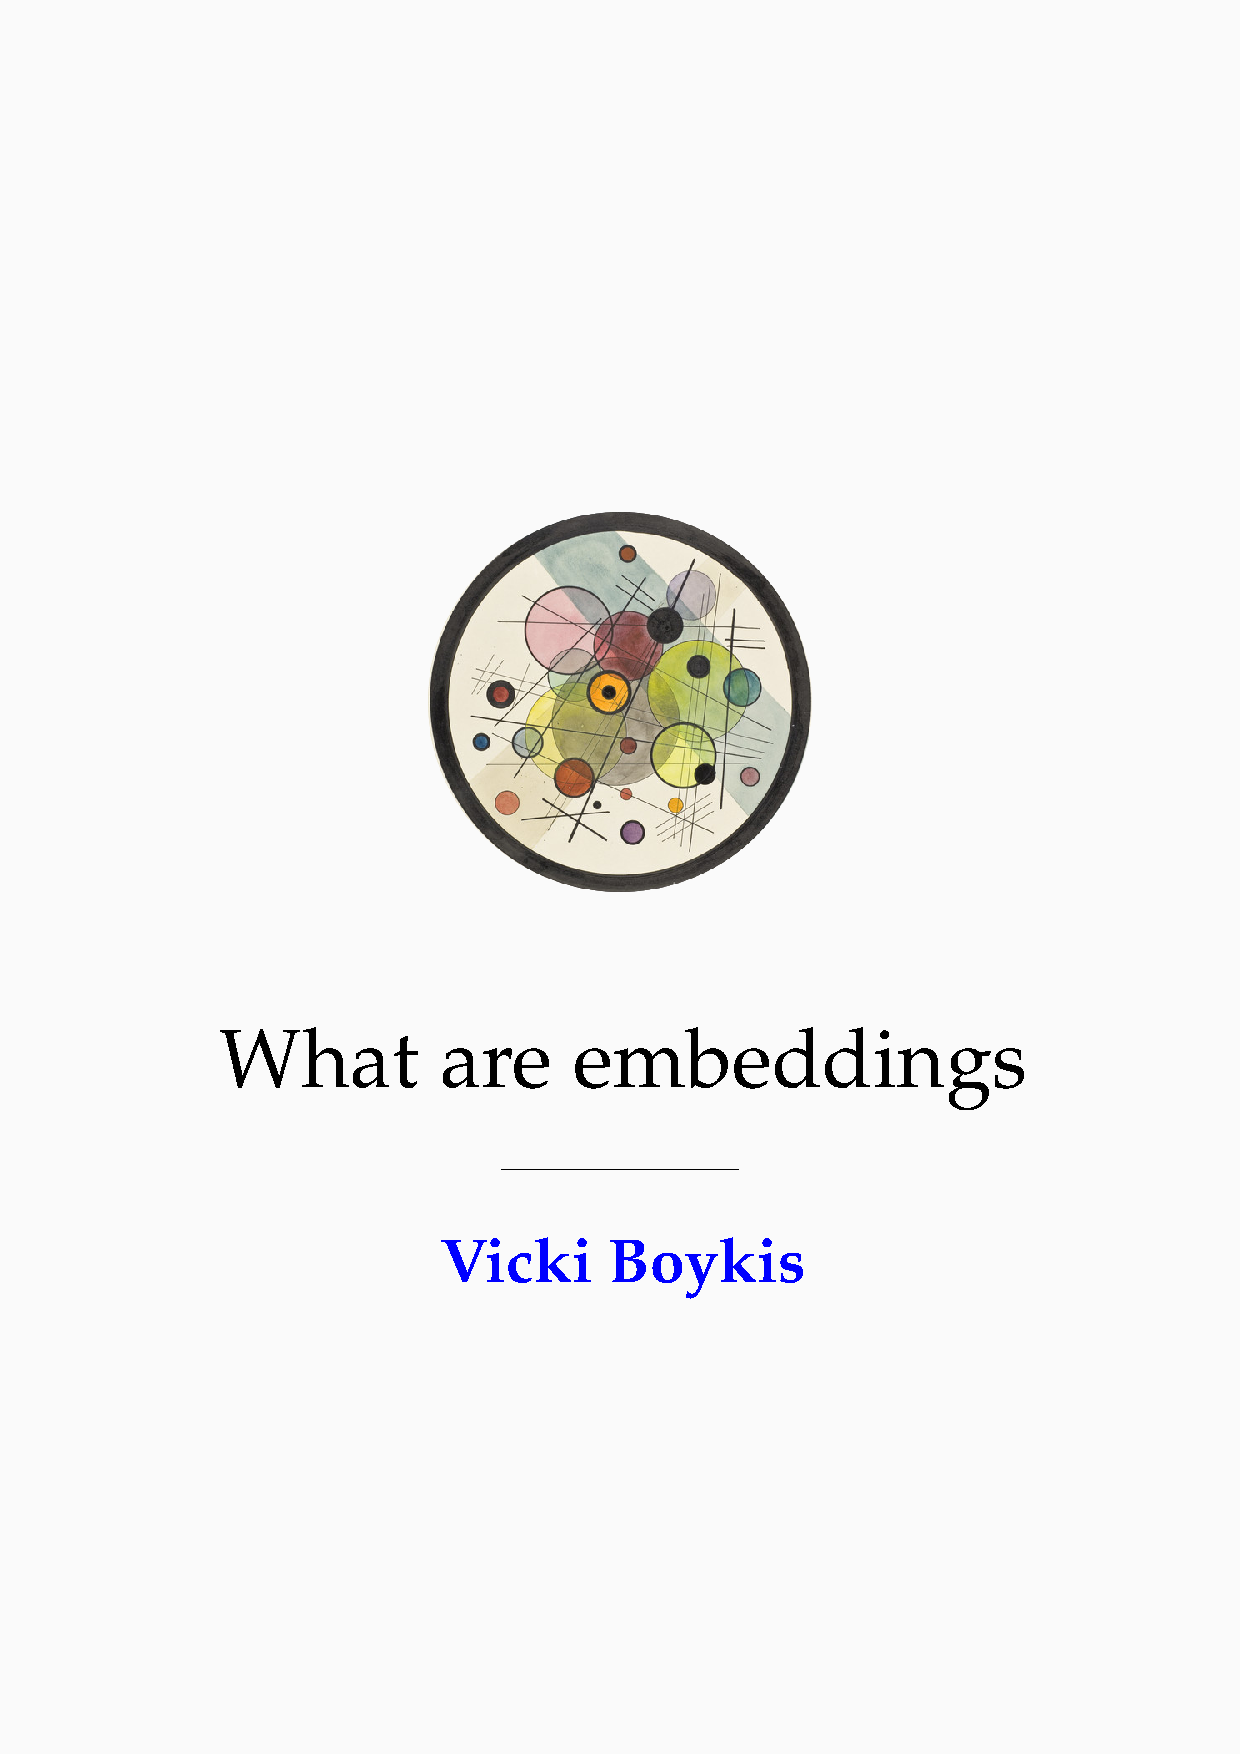
\includegraphics[width=\textwidth]{figures/embeddings.png}}
\caption{Left to right: Embeddings as recommendations in Spotify Radio, in YouTube Video recommendations, in visual recommendations at Pinterest, and as BERT Embeddings in suggested Google search results}
\end{figure}

Given how expensive they can be to generate and how complicated they become to manage, the need to create, store, and manage embeddings has also recently resulted in the explosion of an entire ecosystem of related products, for example, the recent rise in the development of vector databases to facilitate production-ready use of nearest neighbors semantic queries in machine learning systems\footnote{For a survey of the vector database space today, refer to  \href{https://dmitry-kan.medium.com/landscape-of-vector-databases-d241b279f486}{this article}}.

\subsection{Embeddings}
 
\subsubsection{What are embeddings}
The canonical definition of embeddings is that they: 

\begin{itemize}
   \item Transform text to useable computational representations which are structures like vectors, tensors, or graphs\citep{rao2019natural}
  \item Compress input information in the context of a machine learning task, such as summarizing a document or trying to identify tags or labels for social media posts or querying a large text corpus. They reduce the number of dimensions of a given set of input data so we can work with and reason about it better. How that compression happens is highly dependent on the task itself. 
  \item Represent non-vector data as a vector\footnote{Vectors have many definitions but for the purpose of machine learning, we can think of them as simply a list of numbers.  When we complete tasks in machine learning, we perform operations on vectors  that looks like this $vector = [1,2,3,4]$  } so we can compare any two embeddings through a variety of distance measures
  \item Embedding space that's created is context-dependent, meaning that any values embedded in the space have a relationship with one another
\end{itemize}

What do embeddings actually look like? In practice, they’re very large collections of vectors that represent  words, phrases, images, or videos as numbers so they can be used for further processing.   

\begin{figure}[!ht]
    \centering
    \begin{tikzpicture}
        \node[draw, rectangle] (multimodal) at (0,0) [block] {
            \begin{tabular}{c}
                Word \\
                Sentence \\
                Video \\
                Image
            \end{tabular}
        };
        \node[above] at (multimodal.north) {Multi-modal data} [block];

        \node[draw, rectangle, right of=multimodal, xshift=3cm] (embedding) [block] {
            \begin{tabular}{c}
               $[1,2,3]$ \\
               $ [4,5,6]$ \\
               $ [7,8,9]$
            \end{tabular}
        };
         \node[above] at (embedding.north) {Embedding Space} [block];

        \draw[->] (multimodal) -- node[above] {Algorithm } (embedding);
    \end{tikzpicture}
    \caption{The process of embedding.}
    \label{fig:embedding}
\end{figure}

Here is one single embedding, also called a \textbf{vector}.

\begin{equation}
\begin{bmatrix}
1 \\
4 \\
9
\end{bmatrix}
\end{equation}

Usually when we create embeddings, we do it at the level of the character (rare), word (very common), or sentence, image, or audio clip level. For example, here is a truncated view of the embedding for the word "not" in the sentence "Not to beat around the bush, but the butterfly bush is the best flower for hummingbirds." 

\begin{figure}[!ht]
\begin{minted}
[
frame=lines,
framesep=2mm,
baselinestretch=1.2,
fontsize=\footnotesize,
linenos
]{python3}
import torch
from transformers import BertTokenizer, BertModel

# Load pre-trained model tokenizer (vocabulary)
tokenizer = BertTokenizer.from_pretrained('bert-base-uncased')

text = """Not to beat around the bush, 
but the butterfly bush is the best flower for hummingbirds."""

# Lots of BERT code truncated for clarity of this example

print ('Shape is: %d x %d' % (len(embeddings), len(embeddings[0])))

[tensor([ 1.0265e-01, -2.2793e+00, -2.0930e-01,  2.9740e-01, -1.2967e+00,
         -4.9467e-01,  7.1440e-01,  2.1999e+00, -4.0721e-01, -4.2629e-01, ...
         1.5620e+00])

\end{minted}
\caption{Analyzing Embeddings with BERT. See full notebook \href{https://colab.research.google.com/drive/1EIEIBw4i0MxTeH07Nsg47SN1Yy6Ma1qC}{here}}
\end{figure}

And here is a \textbf{tensor}, also known as a \textbf{matrix}\footnote{The difference between a matrix and a tensor is that it's a matrix if you're doing linear algebra and a tensor if you're an AI researcher.}, which is a multidimensional combination of vectors.  

\begin{equation}
\begin{bmatrix}
1 & 2 & 3\\
4 & 5 & 6
\end{bmatrix}
\end{equation}


We'll be returning to this BERT deep learning implementation of embeddings at the end of the document. For now all our energy will be spent building an intuition around what the process of embedding means in a general sense. 

In Systems Thinking, Donella Meadows says, “You think that because you understand “one” that you must therefore understand “two” because one and one make two. But you forget that you must also understand “and.”\citep{meadows2008thinking} In order to understand embeddings, we must understand where they came from and how they came to be, as well as formulate a framework for thinking about them. 

\subsubsection{Three Easy Pieces}
Richard Feymman wrote a book called "Six Easy Pieces" explaining the fundamental concepts in physics. There are, similarly, several fundamental concepts that make up the work of transforming words to numerical representations. 

These show up over and over again, in every fundamental architecture and every NLP-related task\footnote{When we talk about tasks in NLP-based machine learning, we mean very specifically, what the machine learning problem is formulated to do. For example, we have the task of ranking, recommendation, translation, text summarization, and so on.}, no matter how simple the model or how complex the neural network: 

\begin{itemize}
  \item Vectors
  \item Encoding
  \item Probability Distributions
\end{itemize}

As Remi and Andrea Arpaci-Dusseau write in their book about operating systems, "Like any system build by humans, good ideas accumulated in operating systems over time, as engineers learned what was important in their design."\citep{arpaci2018operating} The same is true for today's large language models, even ChatGPT. They did not arise out of thin air, but were built on hundreds of building blocks of ideas over the course of decades.

As we go through the historical context of embeddings, keep this in mind. We'll build our intuition all the way up to BERT, but first we have to start at the very beginning\footnote{Original diagram from  \href{http://mccormickml.com/2019/11/11/bert-research-ep-1-key-concepts-and-sources/}{this excellent guide on BERT}}. 

\begin{figure}[!ht]
\centering
\includegraphics[width=\textwidth]{figures/pyramid.png}
\caption{Pyramid of fundamental concepts building to BERT}
\end{figure}

To build a model that will act as our candidate generator, we need to understand what approaches we can use. When we think about the process of embedding, the high-level mental model we should have is that our machine learning input data is highly-dimensional and grows exponentially with the amount of data we generate, and we are constantly trying to come up with an efficient way to represent it and work with it in lower dimensions.

\subsubsection{History of Embeddings}
Compressing content into lower dimensions as numerical representations is not a new idea in machine learning. Earlier approaches have included one-hot encoding, TF-IDF, LDA \footnote{Used at the \href{https://archive.nytimes.com/open.blogs.nytimes.com/2015/08/11/building-the-next-new-york-times-recommendation-engine/}{New York Times} around 2015} , and PCA and SVM. 

\begin{figure}[H]
    \centering
\begin{forest}
  for tree={
    draw,
    align=center,
    parent anchor=south,
    child anchor=north,
    font=\sffamily,
    edge={->,thick},
    l sep+=20pt,
  }
  [\textbf{Embedding Methods}    [\textbf{Count-based Methods}      [\textbf{TF-IDF}]
      [\textbf{One-Hot Encoding}]
      [\textbf{LSA}]
      [\textbf{LDA}]
    ]
    [\textbf{Prediction-based Methods}      [\textbf{SVM}]
      [\textbf{Word2Vec}]
      [\textbf{BERT}]
    ]
  ]
\end{forest}
     \caption{Embedding Method Solution Space}
\end{figure}


All of these earlier methods have been part of the information retrieval toolbox for decades and have worked extremely well in their respective industrial use-cases. But the usage of embeddings that capture semantic meaning to generate compressed representations of content exploded in popularity after the publication of Google’s Word2Vec paper \citep{mikolov2013efficient}. Building and expanding on the concepts in Word2Vec, the Transformer \citep{vaswani2017attention} architecture, a much more specialized case of calculating context around a given word, really caused embeddings to become a staple of deep learning workflows. 

\begin{figure}[H]
\centering
\includegraphics[width=\linewidth]{figures/embeddings1.png} 
\caption{Embeddings papers in Arxiv by month. \\ \href{https://colab.research.google.com/drive/1W_CIk_aBh7Oz0eKr8ZuWtgi1cj1sKVum}{source}}
\end{figure}


In short, embeddings have become a critical part of machine learning infrastructure for any organization working with large amounts of textual data, and especially for organizations that have large amounts of heterogenous data they need to filter and present to users.  Additionally, there is now a whole ecosystem \footnote{\href{https://github.com/currentslab/awesome-vector-search}{So much vector search}} around storing and creating services that manage embeddings \footnote{We've even gotten to the point where embeddings are a key differentiator in pricing between \href{https://openai.com/pricing}{on-demand ML services}}. As such, it's important to understand their context both as end-consumers and as developers who work on these platforms.

\section{Formulating a machine learning problem}

In order to think about how to to use embeddings, we need to put them into the context of the machine learning problem.As we saw in the last section, machine learning is a process that takes data as input to produce rules for how we should classify something or filter it or recommend it. What happens inside the box of the process? The core of machine learning is the model, which is a set of instructions for how to learn the input data parameters we feed it and output some set of results.

There are generally three categories of machine learning, \textbf{supervised}, where we have training data that can tell us whether the results the model predicted are correct according to some model of the world. The second is \textbf{unsupervised}, where we don't know ahead of time what the answer might be. An example here is clustering of our customer base. A clustering model can detect patterns in your data but won't explicitly label what those patterns are. The third is \textbf{reinforcement learning}  which is separate from these two categories and formulated as a game theory problem: we have an agent moving through an environment and focuses on understanding how to optimally move an agent through a given environment using explore-exploit techniques. We'll focus mostly on supervised learning in this document, with the exception of Word2Vec and PCA, which are unsupervised approaches. 
 
 \begin{figure}[!h]
    \centering
  \begin{tikzpicture}[auto, node distance=2cm]
    \tikzstyle{block} = [rectangle, draw, fill=green!20, text width=6em, text centered, rounded corners, minimum height=4em]
    \tikzstyle{smallblock} = [rectangle, draw, fill=green!20, text width=5em, text centered, rounded corners, minimum height=3em]
    \tikzstyle{line} = [draw, -latex']
    
    % Machine Learning
    \node [block] (ml) {Machine Learning};
    
    % Supervised Machine Learning
    \node [block, below left of=ml, xshift=-3cm, yshift=-0.5cm] (supervised) {Supervised\\Machine Learning};
    
    % SVM
    \node [smallblock, below of=supervised, xshift=-2cm, yshift=-0.5cm] (svm) {SVM};
    
    % Linear Regression
    \node [smallblock, below of=supervised, xshift=0cm, yshift=-0.5cm] (linear) {Regression};
    
    % Neural Networks
    \node [smallblock, below of=supervised, xshift=2cm, yshift=-0.5cm] (neural) {Neural\\Networks};
    
    % Unsupervised Machine Learning
    \node [block, below of=ml, yshift=-1.5cm] (unsupervised) {Unsupervised\\Machine Learning};
    
    % Clustering
    \node [smallblock, below of=unsupervised, xshift=-2cm, yshift=-0.5cm] (clustering) {Clustering};
    
    % Dimensionality Reduction
    \node [smallblock, below of=unsupervised, xshift=2cm, yshift=-0.5cm] (dimensionality) {Dim Reduction};
    
    % Principal Components Analysis
    \node [smallblock, below of=dimensionality, xshift=0.5cm, yshift=-0.5cm] (pca) {PCA};
    
    % Reinforcement Learning
    \node [block, below right of=ml, xshift=3cm, yshift=-0.5cm] (reinforcement) {Reinforcement\\Learning};
    
    % Arrows
    \path [line] (ml) -- (supervised);
    \path [line] (ml) -- (unsupervised);
    \path [line] (ml) -- (reinforcement);
    \path [line] (supervised) -- (svm);
    \path [line] (supervised) -- (linear);
    \path [line] (supervised) -- (neural);
    \path [line] (unsupervised) -- (clustering);
    \path [line] (unsupervised) -- (dimensionality);
    \path [line] (dimensionality) -- (pca);

  \end{tikzpicture}
     \caption{Machine learning approach solution space}
\end{figure}

There are generally three categories of machine learning, \textbf{supervised}, where we have training data that can tell us whether the results the model predicted are correct according to some model of the world. The second is \textbf{unsupervised}, where we don't know ahead of time what the answer might be. An example here is clustering of our customer base. A clustering model can detect patterns in your data but won't explicitly label what those patterns are. The third is \textbf{reinforcement learning}  which is separate from these two categories and formulated as a game theory problem: we have an agent moving through an environment and focuses on understanding how to optimally move an agent through a given environment using explore-exploit techniques. We'll focus mostly on supervised learning in this document, with the exception of Word2Vec and PCA, which are unsupervised approaches. 

\subsection{Formalizing the machine learning model}

The machine learning model, in our case, the \textbf{candidate generator} at its very heart, is a function with a set of learnable\footnote{When we say learnable, we mean that we can learn what the correct inputs into a model are through some kind of iterative process where we feed the model data and see if it improves.} input parameters that takes some set of inputs and gives us an output. 

Supervised machine learning problems are generally formulated the same way. We start with our input data, or a \textbf{corpus} as it's generally known in NLP-related problems. These are our \textbf{features}.  We take two parts of this data as holdout data that we don't feed into the model. The first part, the \textbf{test set}, we use to validate the final model on data it's never seen before. The second, the \textbf{validation set}, we use to check our hyperparameters we use them for validating our hyperparameters during the model training phase. 

\begin{figure}[!ht]
  \includegraphics[width=\linewidth]{figures/model_cycle.png}
  \caption{The cycle of machine learning model development}
\end{figure}

We train our model by initializing it with some set of weights as learnable input parameters, and we input on those weights, usually by minimizing a cost function. The other key part of machine learning is the actual learning part. How do we know our model is any good? We initialize it with some set of values, weights, and we iterate on those weights, usually by minimizing a cost function. The cost function is the generally the difference between our model's predicted value and the real value for that given model.

Let's make this more concrete. For example, let's say that one of our business problems is predicting whether a bird is likely to continue to stay on Flutter or to churn aka leave the platform and disengage\footnote{An extremely common business problem to solve in almost every industry where either customer population or subscription based on revenues is important}, we might have the following inputs: 

\begin{itemize}
  \item How many bird posts the bird has read (we'll call this \mintinline{python}{bird_posts} in our database)
  \item The geographical location of the bird (\mintinline{python}{bird_geo})
  \item How many posts the bird has liked over the past month (\mintinline{python}{bird_likes})
\end{itemize}

\begin{table}[H]
  \centering
    \caption{Tabular Features}
\begin{tabular}{|l|l|l|l|}
\hline
\rowcolor[HTML]{EFEFEF} 
bird\_id & bird\_posts & bird\_geo & bird\_likes \\ \hline
012      & 2           & US        & 5           \\ \hline
013      & 0           & UK        & 4           \\ \hline
056      & 57          & NZ        & 70          \\ \hline
612      & 0           & UK        & 120         \\ \hline
\end{tabular}
\end{table}

\begin{figure}[!ht]
  \includegraphics[width=\linewidth]{figures/function.png}
  \caption{How inputs map to outputs in ML functions \citep{klein2013coding}}
\end{figure}

So here we have a given set of input items, $X$,  which includes all of these items. We have a set of outputs, which in our case will be a binary decision, 1 if the bird is likely to churn, and 0 if it is not, and the algorithm, $f(X) -> y$ that picks points in the best fit model space and iterates through them to pick a final answer for whether it thinks the bird is likely to churn or not, in short defining our business logic. 

Evaluation of the model is at the heart of the modeling process. "First, we feed the training data  to our learning algorithm to learn a model. Second, we predict the labels of our test set. Third we count the number of wrong predictions on the test dataset to compute the model’s prediction  accuracy."\citep{raschka2018model}

\subsection{Machine learning features}
This approach works well for what we consider traditional machine learning approaches which deal with tabular data.  As a general rule, the creation of the correct formulation of input data is perhaps the heart of machine learning. I.e. if we have bad input, we will get bad output. So in all cases, we want to spend our time putting together our input dataset and engineering features very carefully. 

Tabular data is generally any structured data where we do active feature selection and engineering. For example, for a given Flutter user we have their user id, how many posts they've liked, how old the account is, and so on. These are all discrete features that we can feed into our model and learn weights from. 

Something important to note here is that, in our bird interaction data, we have both numerical and textual features. For numerical features, it's easy to perform computation on the numbers. But what do we do with these textual features? How do we compare "US" to "UK"? The process of setting up data correctly to feed into a model is called \textbf{feature engineering}. When we have a single continuous, numerical feature, like “the age of the flit in days”, it’s easy to feed these features into a model. But, when we have textual data, we need to turn it into numerical representations so that we can compare these representations.  

\subsection{Feature Vectors}
We'll talk a lot in this document about features as vectors, and vector and matrix representations of features. It's worth explaining these concepts because they end up being really important in the way we understand embeddings. 

A vector is simply a list of numbers that looks like this $vector = [1,2,3,4]$. We can think of each row in our tabular feature data as a vector.  When we complete tasks in machine learning, we perform operations on vectors. Each of our features is a vector, and a collection of features, or our tabular representation, is a matrix. For example, in this vector, $[1,2,3,4]$, we can see that this particular value is represented by four features. When we create vectors, we can run algorithmic computations over them. 

In linear algebra, vectors are collections of coordinates that tell us where a given point is in space among many dimensions. For example, in two dimensions, we have a point $[1,2]$. In three dimensions, we might have a point $[0,8,0]$ which tells us where that point falls on all three axes directionally. 

\tdplotsetmaincoords{60}{120} 
\begin{tikzpicture} [scale=3, tdplot_main_coords, axis/.style={->,blue,thick}, 
vector/.style={-stealth,red,very thick}, 
vector guide/.style={dashed,red,thick}]

%standard tikz coordinate definition using x, y, z coords
\coordinate (O) at (0,0,0);

%tikz-3dplot coordinate definition using x, y, z coords

\pgfmathsetmacro{\ax}{0.8}
\pgfmathsetmacro{\ay}{0.8}
\pgfmathsetmacro{\az}{0.8}

\coordinate (P) at (\ax,\ay,\az);

%draw axes
\draw[axis] (0,0,0) -- (1,0,0) node[anchor=north east]{$x$};
\draw[axis] (0,0,0) -- (0,1,0) node[anchor=north west]{$y$};
\draw[axis] (0,0,0) -- (0,0,1) node[anchor=south]{$z$};

%draw a vector from O to P
\draw[vector] (O) -- (P);

%draw guide lines to components
\draw[vector guide]         (O) -- (\ax,\ay,0);
\draw[vector guide] (\ax,\ay,0) -- (P);
\draw[vector guide]         (P) -- (0,0,\az);
\draw[vector guide] (\ax,\ay,0) -- (0,\ay,0);
\draw[vector guide] (\ax,\ay,0) -- (0,\ay,0);
\draw[vector guide] (\ax,\ay,0) -- (\ax,0,0);
\node[tdplot_main_coords,anchor=east]
at (\ax,0,0){(\ax, 0, 0)};
\node[tdplot_main_coords,anchor=west]
at (0,\ay,0){(0, \ay, 0)};
\node[tdplot_main_coords,anchor=south]
at (0,0,\az){(0, 0, \az)};
\end{tikzpicture}


One we have one point, we can compare it to other points. So in our case, each row of data tells us where to position each bird in relation to any other given bird based on the combination of features.  And that's really what our features allow us to do. If you think of the first feature as geo, then likes, then posts, you can think of the representation of a bird in three different vectors, or as many vectors as you have features for. 

In order to project our vector into this space, we need to encode them as some sort of numerical value so that modern large-scale models\citep{lakshmanan2020machine} can calculate them as inputs\footnote{There are some models, specifically decision trees, where you don't need to do text encoding because the tree learns the categorical variables out of the box, however implementations differ, for example the two most popular implementations, scikit-learn and XGBoost\citep{altay_2020}, can't.}. 

There are several ways to do this:

\begin{itemize}
  \item Ordinal encoding   
  \item Dummy encoding 
  \item One-Hot encoding
\end{itemize}

Ultimately, in all these cases, what we are doing is creating a new feature that maps to the text feature column but is a numerical representation of the variable so that we can project it into that space for modelling purposes. We'll motivate these examples with simple code snippets from sklearn, the most common library for demonstrating basic ML concepts. 

We'll start with naive, non-model driven-approaches, because that's what the initial solutions to these problems were. 

\section{Historical Embeddings Approaches}
\subsection{Count-based Methods}

\subsubsection{Ordinal encoding}
Ordinal encoding - We have an ordered encoding, for example, "1" is "Cat", "2" is "Dog" and so on. Use this only if the variables have a natural ordered relationship to each other. For example, in this case cat is not "less" than "dog" and so would be incorrectly represented in our model. The same if we we made US 1, UK 2 and so on. 

\begin{table}[H]
 \centering
    \caption{Features Encoded as Numbers}
\begin{tabular}{|l|l|l|l|l|}
\hline
\rowcolor[HTML]{EFEFEF} 
bird\_id & bird\_posts & bird\_geo & bird\_likes & encoded\_bird\_geo \\ \hline
012      & 2           & US        & 5           & 1                  \\ \hline
013      & 0           & UK        & 4           & 2                  \\ \hline
056      & 57          & NZ        & 70          & 3                  \\ \hline
612      & 0           & UK        & 120         & 2                  \\ \hline
\end{tabular}
\end{table}

\begin{figure}[!ht]
\begin{minted}
[
frame=lines,
framesep=2mm,
baselinestretch=1.2,
fontsize=\footnotesize,
linenos
]{python3}
from sklearn.preprocessing import OrdinalEncoder
print(data)
[['US']
 ['UK']
 ['NZ']]
 
# our label features
encoder = OrdinalEncoder()
result = encoder.fit_transform(data)
print(result)
[[2.]
 [1.]
 [0.]]
\end{minted}
\caption{Ordinal Encoding in Scikit-Learn}
\end{figure}

\subsection{Dummy and one-hot encoding}
Dummy encoding is a process that encodes the variables into n-1 categories and creates a new feature for each. So, if we have 3 variables, dummy encoding encodes into 2 dummy variables.  Why would we do this? If the categories are mutually exclusive, as they usually are in point-in-time geolocation estimates, if someone is in the US, we know for sure they're not in the UK and not in NZ.  If we use all these variables and they are very closely related, there is a chance we'll fall into something known as the dummy variable trap. What this means is that we can predict one variable from the others. This generally isn't a risk for geolocation since there are more than 2 or 3 and if you're not in the US, it's not guaranteed that you're in the UK. But  So, for example if we have US = 1, UK = 2, and NZ = 3, and prefer more compact representations, we can use dummy encoding. 

However, many modern ML approaches don't require linear independence and use L1 regularization\footnote{Regularization is a way to prevent our model from overfitting, that is, it can exactly predict based on the training data, but it can't learn new inputs that we show it.} to prune inputs that don't minimize the error, and as such only use one-hot encoding. One-hot encoding takes each row of log features that we have and creates a vector for the text element.  Everywhere the element is present in the sentence, we place a “1” in the vector, and we repeat this for all the other sentence elements we have. What we are doing here is creating a mapping of all the elements in the vocabulary, where “0” indicates a non-match and “1” indicates a match, and seeing how similar various vectors are, where those vectors are either words or sentences or any combination of the two.  

We can represent it this way mathematically, which shows the importance of 1 and 0 in the set. 

\begin{equation}
{1}_A(x) :=
\begin{cases}
1 &\text{if } x \in A, \\
0 &\text{if } x \notin A.
\end{cases}
\end{equation}

\begin{figure}[!ht]
\begin{minted}
[
frame=lines,
framesep=2mm,
baselinestretch=1.2,
fontsize=\footnotesize,
linenos
]{python}
from sklearn.preprocessing import OneHotEncoder
import numpy as np 

enc = OneHotEncoder(handle_unknown='ignore')
data = np.asarray([['US'], ['UK'], ['NZ']])
enc.fit(data)
enc.categories_
# Result: [array(['NZ', 'UK', 'US'], dtype='<U2')]
onehotlabels = enc.transform(data).toarray()
onehotlabels
# Result: 
array([[0., 0., 1.],
       [0., 1., 0.],
       [1., 0., 0.]])
\end{minted}
\caption{One-Hot Encoding in Scikit-learn}
\end{figure}

Now that we've encoded our textual features as numerical, we can feed them into the model and the function we're learning will learn to minimize the loss by predicting correct parameters. We then feed all these features into  the model, the model will return a value within the parameters from 1 to 0 that is a probability that the event, either churn or no-churn, has taken place.  

\begin{equation}
\sum_{i=1}^{D}(x_i-y_i)^2
\end{equation}

his is what's a logistic regression model. Generally these days the machine learning community has converged on using  gradient-boosted decision trees for dealing with tabular data, but we'll stick with the logistic regression example because later on, we'll see that neural networks, which are used to generate embeddings, are a very special case of logistic regression.  

What else can you do with one-hot encoding? You can represent your text features as a numerical vector, just as we did when we created this bit of code 

\begin{figure}[!ht]
\begin{minted}
[
frame=lines,
framesep=2mm,
baselinestretch=1.2,
fontsize=\footnotesize,
linenos
]{python}
array([[0., 0., 1.],
       [0., 1., 0.],
       [1., 0., 0.]])
\end{minted}
\caption{Sparse Vector Representation of Our Feature}
\end{figure}

Now that we have one-hot encoded numerical input data, we can work with it in our recommender system architecture as feature input into our candidate generator.

\subsection{Embeddings as Feature inputs into a recommendation problem}
Now we get to the piece of the puzzle where we go from business logic, to building an app, to the machine learning domain, to formulating a machine learning problem. From a machine learning perspective, the problem we are building towards one of  information retrieval, a vast field with its roots in sifting through scientific publications, legal documents and library records, but then spread to sifting through the reams of news and social content started being generated as more people started using the internet. The first recommendation systems were created to filter messages in email and newsgroups\citep{goldberg1992using}  at the Xerox Palo Alto Research Center. 
	
The goal of information retrieval is to navigate lots of unstructured text documents. Within information retrieval, we have two complementary problems in how we can offer users the correct content in our app: search, and recommendations. Search is the problem of directed\citep{ekstrand2019recommender} information seeking, i.e. we have a query and would like a set of refined results. Recommendations is, as Nick Seaver \citep{seaver2022computing} says, a problem where "man is the query", i.e. based on explicit or implicit information about you, we recommend items that you may prefer based on taste, aka things you're not sure you were looking for because you don't know our full catalog of content, but which match your taste.  Generally these fall into both the supervised and unsupervised space, but we'll focus on formulating a supervised problem for now since it's slightly easier to walk through. 

 First, we take data that’s initially not tabular and create matrix of tabular data so that we can use our words, sentences, or phrases as a feature. Then, we decompose that matrix and perform operations on the component matrices to minimize the distance between certain groups of words. The end-result is our generated recommendation candidates, which we then filter downstream and surface to the user.  Why do we do this? The core of the recommendation problem is to recommend items to the user that are relevant and interesting so the user continues to engage with the platform. 

The best way to think of the difference between tabular and free-form representations as model inputs is this illustration, where we're moving from looking at creating a row of individual features per bird, aka \mintinline{Python}{bird1 = [012,2,"US", 5]}, to a row a string of text. In both cases, each of these are vectors, or a list of values that represents a single bird. This becomes pretty important in understanding compression. 

So in this case, the machine learning problem doesn't take a feature matrix as input: it takes the user information and activity for each given user. Once we get into the recommendation space, and particularly with multimodal (text, video, image, and sound) data, we think about formulating the problem entirely differently. Here, what we're looking to do is to create a function where the parameters are not distinct features, but the coordinates of vectors that are translations for the text into numerical representations, which serve as the parameters, and learning the function\citep{castells2023recommender} becomes a different problem where we're trying to find items that are similar to each other. 

Here’s an example.  We have a Flit that our bird users liked. 

"Hold fast to dreams, for if dreams die, life is a broken-winged bird that cannot fly."

We also have other flits we may or may not want to surface in our bird's feed. 

"No bird soars too high if he soars with his own wings."
“A bird does not sing because it has an answer, it sings because it has a song.” 

How can we recommend similar flits to them in the content stream, and  how would we begin to turn this into a machine learning problem that takes features as input and a prediction as an output, knowing what we know about how to do this already?  First,  we need to turn each word into a feature - we need to hot-encode it and turn it into matrix form, and also create features out of all the other Flits that other birds have liked. Each of these ends up being an entry, just as each of our rows about bird activity was an entry in the last case.  

\begin{figure}[!ht]
\begin{minted}
[
frame=lines,
framesep=2mm,
baselinestretch=1.2,
fontsize=\footnotesize,
linenos
]{python}
from sklearn.feature_extraction.text import CountVectorizer
import pandas as pd

vect = CountVectorizer()

responses = ["Hold fast to dreams, for if dreams die, \
life is a broken-winged bird that cannot fly.", 
"No bird soars too high if he soars with his own wings.", 
"A bird does not sing because it has an answer, it sings because it has a song."]

doc = pd.DataFrame(list(zip(responses)))

td = pd.DataFrame(vects.todense()).iloc[:5]  
td.columns = vect.get_feature_names_out()
term_document_matrix = td.T
term_document_matrix.columns = ['Doc '+str(i) for i in range(1, 4)]
term_document_matrix['total_count'] = term_document_matrix.sum(axis=1)

print(term_document_matrix.drop(columns=['total_count']).head(10))

         Doc 1  Doc 2  Doc 3
an           0      0      1
answer       0      0      1
because      0      0      2
bird         1      1      1
broken       1      0      0
cannot       1      0      0
die          1      0      0
does         0      0      1
dreams       2      0      0
fast         1      0      0
\end{minted}
\caption{Creating a matrix frequency table}
\end{figure}


\subsection{TF-IDF}

Our first approaches to embedding focused on encoding. After the development of one-hot encoding, the next step up was tf-idf, or term frequency-inverse document frequency. The basic concept behind tf-idf is that it will tell you how important a single word is in a corpus by assigning it a weight and, at the same time, downweight common words like "the, a, and." This weight gives us a feature for a single word tf-idf. We take all of our input data that's structured in sentences and break it up into individual words, in a structured commonly called \textbf{bag of words}, and perform counts on its values. 

\begin{figure}[!ht]
\centering
  \includegraphics[width=0.5\columnwidth]{figures/bag_of_words.png}
  \caption{Destructing text that has semantic relationships into a bag of words \href{https://people.cs.georgetown.edu/nschneid/cosc572/f16/05_classification-NB_slides.pdf}{source}}
  \label{fig:timeline}
\end{figure}

Another important representation for bag of words is the term-document representation, which shows us in which documents all the terms appear. This matrix is the input data for many of the early approaches to embedding. 

TF is term frequency, or the number of times a term appears in a document relative to the other terms in the document.

\begin{equation}
\text{tf}{t,d} = \frac{f{t,d}}{\sum\limits_{k}f_{k,d}}
\end{equation}

And IDF is the inverse frequency of the term across all documents that have been ingested. 

\begin{equation}
\mathrm{idf}(t,D) = \log \frac{N}{|{d \in D : t \in d}|}
\end{equation}

It makes a bit more sense when shown in code: 

\begin{figure}[!ht]
\begin{minted}
[
frame=lines,
framesep=2mm,
baselinestretch=1.2,
fontsize=\footnotesize,
linenos
]{python}

import math 

documentA =  ['Hold','fast','to','dreams,', 'for','if','dreams','die,','life','is','a','broken-winged',
'bird','that','cannot','fly.']
 documentB =  ['No','bird','soars','too','high', 'if','he','soars','with','his','own','wings.']

def tf(term: str, document:list[str]) -> flota:
	'''Term frequency of a word in a document  over total words in document'''
	
	term_count = 0
	total_count = 0

	for word in document:
		total_count +=1 
		if word == term:
			term_count += 1

	return (term_count / total_count)

def idf(term:str, doc_list:list[str]) -> float:
	'''Inverse frequency of term across a set of documents'''
	
	total_docs = 0
	total_docs_with_term = 0

	for doc in doc_list: 
		total_docs +=1
		if term in doc:
			total_docs_with_term +=1

	idf = math.log(total_docs / total_docs_with_term)
	return idf

def tf_idf(tf:float, idf:float) -> float:

	tfidf = tf*idf
	print("tf-idf:{:0.3f}".format(tfidf))

tf_bird = tf('bird', documentA)
idf_docs = idf('bird,[documentA, documentB])

tf_idf(tf_bird, idf_docs)
\end{minted}
\caption{Implementation of TF-IDF}
\end{figure}

Or, we can implement it entirely in scikit learn in a few lines of code: 

\begin{figure}[!ht]
\begin{minted}
[
frame=lines,
framesep=2mm,
baselinestretch=1.2,
fontsize=\footnotesize,
linenos
]{python}
from sklearn.feature_extraction.text import TfidfVectorizer
corpus = ["Hold fast to dreams, for if dreams die, life is a broken-winged bird that cannot fly.",
"No bird soars too high if he soars with his own wings.",
"A bird does not sing because it has an answer, it sings because it has a song."]

vectorizer = TfidfVectorizer()
X = vectorizer.fit_transform(corpus)
dict(zip(vectorizer.get_feature_name_outs(), X.toarray()[0]))

{'an': 0.0,
 'answer': 0.0,
 'because': 0.0,
 'bird': 0.14355303576663192,
 'broken': 0.24305641776909384,
 'cannot': 0.24305641776909384,
 'die': 0.24305641776909384,
 'does': 0.0,
 'dreams': 0.4861128355381877,
 'fast': 0.24305641776909384,
 'fly': 0.24305641776909384,
 'for': 0.24305641776909384,
 'has': 0.0,
 'he': 0.0,
 'high': 0.0,
 'his': 0.0,
 'hold': 0.24305641776909384,
 'if': 0.1848506706027212,
 'is': 0.24305641776909384,
 'it': 0.0,
 'life': 0.24305641776909384,
 'no': 0.0,
 'not': 0.0,
 'own': 0.0,
 'sing': 0.0,
 'sings': 0.0,
 'soars': 0.0,
 'song': 0.0,
 'that': 0.24305641776909384,
 'to': 0.24305641776909384,
 'too': 0.0,
 'winged': 0.24305641776909384,
 'wings': 0.0,
 'with': 0.0}

\end{minted}
\caption{Implementation of TF-IDF in Scikit-learn}
\end{figure}

Inverse document frequency is a measure of whether the word is common or not across the documents.  We can see that fly, hold, and die are important because they are rare across the documents and therefore interesting to us. 

The way the equations are formulated are meant to do several things: 

\begin{itemize}
  \item Uprank term frequency when it occurs many times in a small number of documents
  \item Downrank term frequency when it occurs many times in many documents, aka is not relevant
  \item Really downrank the term when it appears across your entire document base\citep{schutze2008introduction}. 
\end{itemize}

There are numerous ways to calculate and create weights for TF-IDF , but what we get in the end is a score for each word that tells us where that word is in relation to each other word in our set, aka our entire set of Flits. Let's say again that we have our original bird quote, and that the quote is one in a set of a million quotes just like it from other Flits. We can figure out how common each word is in the set of all possible flits and get a weighted score for the entire sentence. In other words, we're creating a dense vector for each word entry in the set. 

And, what we are now doing is creating the representation of our entire set of flits as vectors in a common vector space. Now, once we've converted all our words to vectors and each given Flit has a vector, we can do vector-based comparisons using dot products by comparing the cosine similarity of those two vectors. The higher the cosine similarity is for two documents, the better. 

Cosine similarity is a key metric in any machine learning models where we're trying to ascertain the closeness of two items, that is to say, which items we should recommend.  

\begin{equation}
\mathrm{similarity}(\vec{a}, \vec{b}) = \frac{\vec{a} \cdot \vec{b}}{|\vec{a}| |\vec{b}|} = \frac{\sum\limits_{i=1}^{n} a_i b_i}{\sqrt{\sum\limits_{i=1}^{n} a_i^2} \sqrt{\sum\limits_{i=1}^{n} b_i^2}}
\end{equation}

\begin{figure}[!ht]
\begin{minted}
[
frame=lines,
framesep=2mm,
baselinestretch=1.2,
fontsize=\footnotesize,
linenos
]{python}
v1 = [0,3,4,5,6]
v2 = [4,5,6,7,8]

def dot(v1, v2):
	dot_product = sum((a * b) for a,b in zip(v1,v2))
	return dot_product

def cosine_similarity(v1, v2):
	'''
	(v1 dot v2)/||v1|| *||v2||)
	'''
	products = dot(v1,v2)
	denominator = ( (dot(v1,v1) **.5) * (dot(v2,v2) ** .5) )
	similarity = products / denominator
	return similarity

print(cosine_similarity(v1, v2))
# 0.9544074144996451
\end{minted}
\caption{Implementation of cosine similarity}
\end{figure}


Or, once again, simply

\begin{figure}[!ht]
\begin{minted}
[
frame=lines,
framesep=2mm,
baselinestretch=1.2,
fontsize=\footnotesize,
linenos
]{python}
from sklearn.metrics import pairwise

v1 = [0,3,4,5,6]
v2 = [4,5,6,7,8]

# need to be in numpy data format
pairwise.cosine_similarity([v1],[v2])
# array([[0.95440741]])

\end{minted}
\caption{Implementation of cosine similarity}
\end{figure}

TF-IDF was introduced in the 70s, and  worked really well for a long time and still does in many cases.  For example, one of the most popular and most-used search functions, BM25, uses TF-IDF as a baseline \citep{schutze2008introduction} as a default search strategy in Elasticsearch/Opensearch \footnote{You can check how Elasticsearch implements BM25 \href{https://www.elastic.co/blog/practical-bm25-part-1-how-shards-affect-relevance-scoring-in-elasticsearch}{here}}.

It extends tf-idf to develop a probability associated with the probability of relevance for each pair of words in a document and it is still being applied in neural search today \citep{svore2009machine} .  


\subsection{Moving towards dense representations}
So far, you may be noticing a pattern with all of these encoding methods. First, we take data that’s unstructured and create a matrix of tabular data so that we can use our words, sentences, or phrases as a feature. 

Generally, when we work on text problems, we’re trying to understand which words, phrases, or concepts are similar to each other. Within the problem space of recommendations, we are trying to understand which of our site users are similar to each other, and which items are similar to each other, so that we can recommend content that users will like based on either their item history or the user history of users similar to them. 

For example, a user might have liked one or two flits.  We don’t have access to the ratings of all of their flits, so what we do is compressing the item-user preference space and filter down the possible list of candidates based on candidates that are closest to our given flit while minimizing the error. 

So, when we perform embedding in the context of recsys, we are looking not to create neighborhoods from words, but from items and users, based on the activity of those users on our platform.  This is the solution to the problem of “how do we recommend Flits that are similar to flits that the user has liked.” This is just a special case of creating embeddings from a single feature, and this process takes place through collaborative filtering. Then, we decompose that matrix and perform operations on the component matrices to minimize the distance between certain groups of words. Once we started doing this in NLP, we found we could also apply this problem to the space of recommendations, which looks at the latent space of a given item and recommends similar ones, also based on either text, image, or video input.  

There are many approaches to collaborative filtering, a (simpler) neighborhood-based approach,  which looks at weighted averages of user ratings and computes the adjusted Pearson correlation, or cosine similarity, between users. This results in something we’ve said before that we don’t want - sparse matrices- which don’t give us a lot of information about users and items we don’t know about. 

Then, there is the machine learning approach, which we’ll focus on here, which can be any number of approaches from SVD and LDA, to matrix factorization,  which we’ll focus on here. 

There is a problem with the vectors we created in one-hot encoding: they are sparse. A sparse vector is one that is mostly populated by zeroes with a few values thrown in. They are sparse because most sentences don't contain all the same words as other sentences. For example, in our Flits, we might encounter the word "bird" in two sentences simultaneously, but the rest of the words will be completely different. 

\begin{figure}[!ht]
\begin{minted}
[
frame=lines,
framesep=2mm,
baselinestretch=1.2,
fontsize=\footnotesize,
linenos
]{python}
sparse_vector = [1,0,0,0,0,0,0,0,0,0]
dense_vector = [1,2,2,3,0,4,5,8,8,5]
\end{minted}
\caption{The two types of vectors}
\end{figure}


What we'd like, instead is to create dense vectors, which will  give us more information about the data, the most important of which is accounting for the weight of a given word in proportion to other words. This is where we leave one-hot encodings and move into approaches that are meant to solve for this sparsity and encode everything into a dense vector space. Dense vectors are just vectors that have mostly non-zero values. They take up more room in memory, but they avoid a number of problems that one-hot encodings have: They avoid the cold-start problem, and they allow us to map all elements into a highly-dimensional space. We call these dense representations dynamic representations\citep{Wang2020FromST}. 

\subsection{Model-based methods}
\subsubsection{PCA}

Around the same time that tf-idf was becoming popular, two other approaches from linear algebra started becoming used fairly frequently for dimensionality reduction: principal components analysis(PCA) and singular value decomposition(SVD).  SVD is a general dimensionality reduction technique used across a number of problem spaces, but which can also be applied in the context of text embeddings. The difference between the two is often tenuous and confusing (people admitted as much in the 80s! \cite{gerbrands1981relationships}), and for the purposes of this survey paper we won't delve too deeply except to say that PCA can often be implemented using SVD \footnote{\href{https://scikit-learn.org/stable/modules/generated/sklearn.decomposition.PCA.html}{This is how it's implemented in the scikit-learn package}} which decomposes a matrix into its composing parts. 

PCA uses the same initial input feature matrix as one-hot encoding, but, whereas one-hot encoding simply converts the text features into numerical features that you can work with, PCA actually performs compression.  SVD, a dimensionality reduction method that works best on sparse matrices like the kind we end up with with respect to text data,  acts on the initial matrix. It decomposes the initial data matrix, or factors it, into three component matrices, one made up of the initial users, one of the items (the features), and one of the strength of the latent factors. It then uses the component matrices to create linear combinations of features that are the largest differences from each other and which are directionally different based on the variance of the clusters of points from a given line.   Those clusters represent the “feature clusters” of the compressed features.  
The resulting model is a projection of all the words, clustered into a single space based on these dimensions. If we were to cluster-map our input data, it might look something like this. 


As you can see from the chart, it’s not clear what the “components” mean, but it’s clear that the clusters of words, aka features, are \textbf{semantically similar}, that is they are close to each other in meaning\footnote{There are many definitions of semantic similarity - what does it mean for "king" and "queen" to be close to each other? - but a high-level approach involves using original sources like thesauri and dictionaries to create a structured knowledge base and offer a structured representation of terms and concepts based on nodes and edges, aka how often they appear near each other. \cite{handrasekaran2021evolution}}


To put this in the context of our initial dataset, let's say we again have our Flutter bird data, except now we have it formulated as input data rather than the raw quotes: 


\setlength\tabcolsep{0pt}

\begin{table}[H]
\begin{tabular*}{\linewidth}{@{\extracolsep{\fill}} cccccc }
\cellcolor[HTML]{C0C0C0}flit\_id & \cellcolor[HTML]{C0C0C0}flit\_content                                                                                                         &  \\
98232                          & Hold fast to dreams, for if dreams die, life is a broken-winged bird that cannot fly.  \\
98234                          & No bird soars too high if he soars with his own wings. &  \\
98235                          & A bird does not sing because it has an answer, it sings because it has a song. & 
\end{tabular*}
\end{table}

We consider each Flit as a document, and we create a term-frequency  document, just as we do when we perform tf-idf:

\begin{figure}[!ht]
\begin{minted}
[
frame=lines,
framesep=2mm,
baselinestretch=1.2,
fontsize=\footnotesize,
linenos
]{python}
from sklearn.feature_extraction.text import CountVectorizer
import pandas as pd
vect = CountVectorizer()

responses = ["Hold fast to dreams, for if dreams die, life is a broken-winged bird that cannot fly.", "No bird soars too high if he soars with his own wings.", 
"A bird does not sing because it has an answer, it sings because it has a song."]

doc = pd.DataFrame(list(zip(responses)))

td = pd.DataFrame(vects.todense()).iloc[:5]  
td.columns = vect.get_feature_names_out()
term_document_matrix = td.T
term_document_matrix.columns = ['Doc '+str(i) for i in range(1, 4)]
term_document_matrix['total_count'] = term_document_matrix.sum(axis=1)

print(term_document_matrix.drop(columns=['total_count']).head(10))

         Doc 1  Doc 2  Doc 3
an           0      0      1
answer       0      0      1
because      0      0      2
bird         1      1      1
broken       1      0      0
cannot       1      0      0
die          1      0      0
does         0      0      1
dreams       2      0      0
fast         1      0      0
\end{minted}
\caption{Creating a matrix frequency table}
\end{figure}


Where one-hot encoding creates a sparse matrix, PCA creates a dense matrix that  allows us to plot individual items (images, words, etc.) as combinations of these two components on an axis and reduces the risk of the curse of dimensionality. Because PCA acts on each combination of features to generate the two dimensions, it becomes immensely computationally expensive.  This meant that these early methods worked well for smaller datasets, like many of the ones used in traditional NLP research,  but as datasets continued to grow and data formats continued to explode, they didn’t quite work anymore. 


\subsubsection{LSA and LDA}
Because PCA acts on each combination of features to compress, it becomes immensely computationally expensive.  This meant that these early methods worked well for smaller datasets, like many of the ones used in traditional NLP research,  but as datasets continued to grow and data formats continued to explode, they didn’t quite work anymore.   

Other approaches grew out of tf-idf and PCA to try to address their limitations, including latent semantic analysis, LSA and latent dirichlet analysis, LDA\cite{cvitanic2016lda}.  Both of these approaches include the word-document matrix that we built intuitively in the last section. The principle behind both is that words that occur close together more frequently have more important relationships.  LSA uses the same word weighting that we used for tf-idf and looks to combine that matrix into a lower rank matrix, a cosine similarity matrix. In the matrix, the values for the cells range from [-1,1], where -1 represents documents that are complete opposits and 1 means the documents are identical. 

LDA takes a slightly different approach. Although it uses the same matrix for input, it instead outputs a matrix where the rows are words and columns are documents. The values, instead of being cosine similarity, are the numerical value for the topic that the intersection of the word and document provide.  The assumption is that any sentence you input will contain a collection of topics, based on proportions, and that there are a number of topics that we can use to classify. We initialize the algorithm by assuming that there is a non-zero probability that each word could appear in a topic. 

But, instead of trying to minimize the distance from groups of words to any single given principal components, LDA initially assigns words to topics at random, and then iterates until it converges to a point where it maximizes the probability for assigning a current word to a current topic.  In order to do this word-to-topic mapping, LDA generates an embedding that creates a space of clusters of words or sentences that work together semantically. 

\subsection{Limitations of traditional approaches}
 
 All of these try to address the problem of generating semantic meaning from words in various ways. Ultimately what they're trying to get at is an understanding of the latent space - the relationships between words that are not explicitly stated but that we can pull out based on how we model the data. However, in all these cases, we start to run into two problems as our corpus grows: the curse of dimensionality and engineering compute scale. 
 
 \subsubsection{The curse of dimensionality}

Something you may have noticed is that, as we one-hot encode more features, our tabular data set grows proportionally in size. What happens once we have 181 countries? We'll have to encode each of them (or each-1) into their own vector representations.

If the model we want to create is based mostly on text, as would be the case if we want to do anything related to understanding what kind of content to recommend to other birds? But think about how large this computation would need to be to understand an entire vocabulary, for example thousands of birds posting millions of messages every day. We'd have to learn an infinite number of features, which would be really inefficient.

But, whereas our input vectors for "classical" tabular machine learning is only three entries wide, text data effectively has a dimensionality of the number of written words in existence and image data has a dimensionality of height times width in pixels, for each given image. Then, there is also video data, on the rise with the popularity of apps such as TikTok, songs, podcasts, and a number of combinations of those media across apps.  In this case, we have 28 features, one for each word in the sentence, assuming we don't remove and process stop words, a common task in NLP.  How can we create a model that has 28 features? That's fairly simple if tedious - we encode each word as a numerical value. 

Not only will it be hard to run computations over a potentially infinite set, once you start generating a large number of features (columns), you start running into the \textbf{curse of dimensionality}, which means that, the more features you accumulate, the more data you need in order to accurately statistically confidently say anything about them, which results in models that may not accurately represent your data\citep{houle2010can}. 


\begin{table}[h!]
    \centering
    \caption{One-hot encoding and the growing curse of dimensionality}
\begin{tabular}{|l|l|l|l|l|l|l|l|}
\hline
\rowcolor[HTML]{EFEFEF} 
flit\_id & username & bad & days & happen & to & everyone & but \\ \hline
9823420  & colibri  & 1   & 1    & 1      & 1  & 1        & 1   \\ \hline
9823421  & colibri  & 1   & 0    & 0      & 0  & 0        & 0   \\ \hline
\end{tabular}
\end{table}

One-hot encodings for textual features are simple to implement, but they have a large problem: each time our vocabulary increases by one word, we need to add a column. This means that one-hot encodings, in terms of computing performance, are \begin{math}O(n)\end{math} in the worst case complexity, which means that if your text is a corpus of a million words, you'll get to a million columns, or vectors, each of which will be sparse, since most sentences will not contain the words of other sentences.   

What happens in practice with tf-idf is, not only does it become hard to compute, but it becomes hard to build a model with an extremely sparse feature base. What TF-IDF ignores is the relationship of the words in position to each other. And that turns out to be really important in context. So what happens when we have really large documents is that the performance of td-idf starts to degrade in returning relevant search results to the user. 
 
  \subsubsection{Computational complexity}
  
%Second, something that's important in machine learning is not only the performance of our algorithm, but how quickly it performs in the context of production environments, or the system's efficiency. Systems efficiency can be measured in many ways, and it is critical in any well-performing system to find the performance bottleneck that leads to latency, or the time spent waiting before an operation is  performed\citep{gregg2014systems}. If you have a recommendation system in production, you cannot risk showing the user an empty feed. If you have a search system, you cannot risk the results taking more than a few milliseconds to return, particularly in e-commerce settings \cite{arapakis2014impact}.  From the holistic systems perspective then, we can also have latency in how long it takes to generate data for a model, read in data, and train the model. 

The two big drivers of latency are: 

\begin{itemize}
  \item I/O processing - You can only send as many items over the network as your network speed allows
  \item CPU processing - you can only process as many items as you have memory available to you in any given system\footnote{there has been \href{https://benhoyt.com/writings/io-is-no-longer-the-bottleneck/}{discussion} over the past few years on whether IO or CPU are really the bottleneck in any modern data-intensive application.}
\end{itemize}

We can measure and profile the performance of any code we write using big O notation, which will classify an algorithm (in this case, a code block not specific to machine learning)'s runtime.  There are programs that perform worse and those that perform better based on the number of elements the program processes. 

Generally, tf-idf performs well in terms of identifying key terms in the document. However, since the algorithm processes all the elements in a given corpus, the time complexity grows for both the numerator and the denominator in the equation and overall, the time-complexity of computing the TF-IDF weights for all the terms in all the documents is $O(Nd)$, where $N$ is the total number of terms in the corpus and $d$ is the number of documents in the corpus. Additionally, because TF-IDF creates a matrix, what you end up doing is processing enormous state matrices. For example, if you have ~100k documents and need to store frequency counts and features for the top 5k words appearing in those documents, , you get a matrix of size $100000*5000$

This linear time complexity growth becomes an issue when you're trying to process millions or hundreds of millions of tokens from documents at once, which happened in the 1990s with the advent of the internet.  As more and more people came online and storage became cheap, the amount of information and audit trails they started to generate also became exponentially enormous.  
\subsubsection{SVM}
The first prediction-based methods were "shallow" - that is models that have only one layer\citep{collobert2008unified}. Support Vector Machines featured prominently in this space. SVMs are a way to classify points that are linearly separable by a hyperplane. HOwever, as in other cases, when you reach high dimensions, SVMs completely fail to work with sparse data. 

Examples of tasks that we can use that will generate supervised data include next word prediction, predicting the missing word in a given sequence, and predicting words that occur in a window. When we think of the classical word embedding inference task, we can think of autocorrect when we're typing on our phones. We type a word, and it's the job of the autocorrect to predict the correct word based on both the word itself and the surrounding context in the sentence. It therefore needs to learn a vocabulary and embeddings that will give it probabilities that it is selecting the correct word. This is a great motivation for Word2Vec. 

\subsubsection{Word2Vec}

From newsgroups to emails, and finally, to public internet text, we began to generate a lot of digital exhaust and companies collected it in the form of append-only logs\citep{kreps2014heart}, a sequence of records ordered by time, that's configured to continuously append records.\footnote{Jay Kreps' \href{https://engineering.linkedin.com/distributed-systems/log-what-every-software-engineer-should-know-about-real-time-datas-unifying}{canonical posts} on how logging works are a must-read} . 

Companies started emitting, keeping, and using those endless log streams for data analysis and machine learning. All of a sudden, the algorithms that had worked well on a collection of 1000 documents didn't work well when our corpuses grew exponentially. In order to get around the limitations of earlier textual approaches, in 2013, researchers at Google, one of the first companies dealing with data at scale, came up with an elegant solution to this problem using the then-new field of neural networks, called Word2Vec\citep{mikolov2013efficient}.  

So far, we've moved from simple heuristics like one-hot encoding, to machine learning approaches like LSA and LDA that look to learn a dataset's modeled features.  Previously, all the approaches to embedding focused on generating sparse vectors much like our original example of one-hot encodings. A sparse vector gives an indication that two words are related, but not that there is a semantic relationship between them. For example, “The dog changed the cat” and “the cat chased the dog” would have the same distance in the vector space, even though they’re two completely different sentences. Word2Vec picks up explicitly where LDA and LSA leave off and creates a deep learning representation of our semantic embedding space. 

Word2vec itself is actually a group of models that has several implementations, each of which focus not on the words themselves, but transforming the entire dataset into vector representations and, more importantly, focusing  not only on the inherent labels of individual words, but on the relationship between those representations. 
  
It uses two approaches - CBOW (continuous bag of words) and skipgrams, both of which generate those dense vectors of embeddings we'd like to have, where each user/feature combination has something meaningful, which we like a lot more than sparse vectors because they give us more signal about our data. 
 
Both of these implementations figure out the probability that a given word is related to a given corpus. The goal of the Word2Vec model is to set the parameters that maximize the probability\citep{goldberg2014word2vec}. 

\begin{equation}
\arg\max_\theta \prod_{w\in Text}\left[\prod_{c \in C(w)} p(c|w;\theta)\right]
\end{equation}

If we maximize this, we will get good embeddings. In both CBOW and skipgrams, we start with  an input layer of our corpus. We translate that layer embeddings, and, using these embeddings, predict the likelihood that the word we're predicting the correct word. 
 
\def\layersep{2.5cm}

\begin{tikzpicture}[shorten >=1pt,->,draw=black!50, node distance=\layersep]
    \tikzstyle{every pin edge}=[<-,shorten <=1pt]
    \tikzstyle{neuron}=[circle,fill=black!25,minimum size=17pt,inner sep=0pt]
    \tikzstyle{input neuron}=[neuron, fill=green!50];
    \tikzstyle{output neuron}=[neuron, fill=red!50];
    \tikzstyle{hidden neuron}=[neuron, fill=blue!50];
    \tikzstyle{annot} = [text width=4em, text centered]

    % Draw the input layer nodes
    \foreach \name / \y in {1,...,4}
    % This is the same as writing \foreach \name / \y in {1/1,2/2,3/3,4/4}
        \node[input neuron, pin=left:Input \#\y] (I-\name) at (0,-\y) {};

    % Draw the hidden layer nodes
    \foreach \name / \y in {1,...,5}
        \path[yshift=0.5cm]
            node[hidden neuron] (H-\name) at (\layersep,-\y cm) {};

    % Draw the output layer node
    \node[output neuron,pin={[pin edge={->}]right:Output}, right of=H-3] (O) {};

    % Connect every node in the input layer with every node in the
    % hidden layer.
    \foreach \source in {1,...,4}
        \foreach \dest in {1,...,5}
            \path (I-\source) edge (H-\dest);

    % Connect every node in the hidden layer with the output layer
     \foreach \source in {1,...,5}
        \path (H-\source) edge (O);

    % Annotate the layers
    \node[annot,above of=H-1, node distance=1cm] (hl) {Hidden layer};
    \node[annot,left of=hl] {Input layer};
    \node[annot,right of=hl] {Output layer};
\end{tikzpicture}

Let's start from the beginning, our input data.  In this case, our corpus are all of the Flits we've collected. We first need to process them as input into our model. 

\begin{figure}[H]
\begin{minted}
[
frame=lines,
framesep=2mm,
baselinestretch=1.2,
fontsize=\footnotesize,
linenos
]{python3}
responses = ["Hold fast to dreams, for if dreams die, life is a broken-winged bird that cannot fly.", "No bird soars too high if he soars with his own wings.", 
"A bird does not sing because it has an answer, it sings because it has a song."]
\end{minted}
\caption{Our Word2Vec input dataset}
\end{figure}


To create data for PyTorch, we can use DataLoader, or Vocabulary, which splits our text into tokens and tokenizes it for processing.   For each line in the file, we generate tokens by performing all of our common NLP preprocessing steps: splitting the text into single items, removing whitespace and punctuation, and lowercasing. 

This kind of processing pipeline is extremely common in NLP and spending time on it is extremely critical so that we get clean, correct input data, and typically includes\citep{naseem2021comprehensive}: 

\begin{itemize}
  \item Tokenization - transforming a sentence or a word into its component character by splitting it
  \item Removing noise - Including URLs, punctuation, and anything else in the text (JSON representations) that is not relevant to the task at hand
  \item Word segmentation
  \item Correcting spelling mistakes
  \item Correcting spelling mistakes
\end{itemize}


\begin{figure}[!ht]
\begin{minted}
[
frame=lines,
framesep=2mm,
baselinestretch=1.2,
fontsize=\footnotesize,
linenos
]{python3}
class TextPreProcessor:
    def __init__(self) -> None:

        # TODO: create utility class for reading relative paths across the project
        self.input_file = "word2vec_input.csv"

        # TODO: split into training and test set

    def generate_tokens(self):

        with open(self.input_file, encoding="utf-8") as f:
            for line in f:
                line = line.replace("\\", "")  # Strip extra \\ in input text
                yield line.strip().split()

    def build_vocab(self) -> Vocab:

        vocab = build_vocab_from_iterator(
            self.generate_tokens(), specials=["<unk>"], min_freq=100
        )
        return vocab
\end{minted}
\caption{Our Word2Vec input dataset}
\end{figure}


Initially, we create our one-hot encoded word to term dictionary: 

\begin{figure}[H]
\begin{minted}
[
frame=lines,
framesep=2mm,
baselinestretch=1.2,
fontsize=\footnotesize,
linenos
]{python3}
In [11]: data = np.asarray([["Hold fast to dreams, for if dreams die, life is a 
    ...: broken-winged bird that cannot fly.",
    ...: "No bird soars too high if he soars with his own wings.",
    ...: "A bird does not sing because it has an answer, it sings because it has
    ...:  a song."]]
    ...: )

In [12]: enc.fit(data)
Out[12]: OneHotEncoder(handle_unknown='ignore')

In [13]: onehotlabels = enc.transform(data).toarray()

In [14]: onehotlabels
Out[14]: array([[1., 1., 1.]])
\end{minted}
\caption{Word2Vec CBOW implementation in Pytorch}
\end{figure}

Then, we create a mapping of each word to a dictionary entry and a dictionary entry to each word. This is known as bijection. The goal is to be able to map back and forth. 

In many ways, Embeddings resemble hash maps and also have their performance characteristics ($O(1)$ retrieval and insert time), which is why they can scale easily when other approaches cannot. 

In the embedding layer, Word2Vec where each value in the vector represents the word on a specific dimension, and more importantly, unlike many of the other methods, the value of each vector is in direct relationship to the other words in the input dataset.

We pick a sliding window, in our case, 2 words before, and 2 words after, and try to infer what the actual word is. This is called the context vector, and in other cases, we'll see that it's called attention. You'll notice that this approach is different than building and looking at the entire matrix - we care about the wrods surrounding the word. For example, if we have the phrase "No bird [blank] too high", we're trying to predict that the answer is "soars" with a given softmax probability, aka ranked against other wrods. Once we have the context vector, we look at what the loss is, aka the difference between the true word and the predicted word, and then we continue. 

\begin{figure}[H]
\begin{minted}
[
frame=lines,
framesep=2mm,
baselinestretch=1.2,
fontsize=\footnotesize,
linenos
]{python3}
class CBOW(torch.nn.Module):
    def __init__(self):  # we pass in vocab_size and embedding_dim as hyperparams
        super(CBOW, self).__init__()
        self.num_epochs = 3
        self.context_size = 2  # 2 words to the left, 2 words to the right
        self.embedding_dim = 100  # Size of your embedding vector
        self.learning_rate = 0.001
        self.device = torch.device('cuda' if torch.cuda.is_available() else 'cpu')

        self.vocab = TextPreProcessor().build_vocab()
        self.word_to_ix = self.vocab.get_stoi()
        self.ix_to_word = self.vocab.get_itos()
        self.vocab_list = list(self.vocab.get_stoi().keys())
        self.vocab_size = len(self.vocab)

        self.model = None

        self.model_path = 'model.ckpt'

        # out: 1 x embedding_dim
        self.embeddings = nn.Embedding(
            self.vocab_size, self.embedding_dim
        )  # initialize an Embedding matrix based on our inputs
        self.linear1 = nn.Linear(self.embedding_dim, 128)
        self.activation_function1 = nn.ReLU()

        # out: 1 x vocab_size
        self.linear2 = nn.Linear(128, self.vocab_size)
        self.activation_function2 = nn.LogSoftmax(dim=-1)
\end{minted}
\caption{Word2Vec CBOW implementation in Pytorch}
\end{figure}

We then build our embedding layer which gives us the ability to perform lookups later on down the line. The embedding layer is just a lookup table\footnote{\href{https://pytorch.org/docs/stable/generated/torch.nn.Embedding.html}{Embedding Layer PyTorch documents}} that matches a word to the corresponding word vector on an index by index basis. In this way, the Embedding layer is like a one-hot encoded matrix, This layer is initialized to a set of random weights, which we next pass onto the linear layer. 

We activate the linear layer with a ReLu activation function, which decides whether a given weight is important or not. In this case, ReLu squashes all the negative values we initizlie our embeddings layer with down to zero since we can't have inverse word relationships, and we perform linear regression by learning the weights of the model of the relationship of the words. 

The way we train this model is through context windows. For each given word in the model, we create a sliding window that includes that word and 2 words before it, and two words after it. Then, for each batch we see what the loss is, i.e. the difference between the real word and the word that we predicted should be there given the context window, and we minimize it. At the end of each epoch, or pass through the model, we pass the weights, or backpropogate them, back to the linear layer,and then again, update the embeddings table with the distance between the words. 
 
\begin{figure}[H]
\begin{minted}
[
frame=lines,
framesep=2mm,
baselinestretch=1.2,
fontsize=\footnotesize,
linenos
]{python3}

def make_context_vector(self, context, word_to_ix) -> torch.LongTensor:
    """
    For each word in the vocab, find sliding windows of [-2,1,0,1,2] indexes
    relative to the position of the word
    :param vocab: list of words in the vocab
    :return: torch.LongTensor
    """
    idxs = [word_to_ix[w] for w in context]
    tensor = torch.LongTensor(idxs)


def train_model(self):

    # Loss and optimizer
    self.model = CBOW().to(self.device)
    optimizer = optim.Adam(self.model.parameters(), lr=self.learning_rate)
    loss_function = nn.NLLLoss()

    logging.warning('Building training data')
    data = self.build_training_data()

    logging.warning('Starting forward pass')
    for epoch in tqdm(range(self.num_epochs)):
        # we start tracking how accurate our intial words are
        total_loss = 0

        # for the x, y in the training data:
        for context, target in data:
            context_vector = self.make_context_vector(context, self.word_to_ix)

            # we look at loss
            log_probs = self.model(context_vector)

            # we compare the loss from what the actual word is related to the probaility of the words
            total_loss += loss_function(
                log_probs, torch.tensor([self.word_to_ix[target]])
            )

        # optimize at the end of each epoch
        optimizer.zero_grad()
        total_loss.backward()
        optimizer.step()

        # Log out some metrics to see if loss decreases
        logging.warning("end of epoch {} | loss {:2.3f}".format(epoch, total_loss))

    torch.save(self.model.state_dict(), self.model_path)
    logging.warning(f'Save model to {self.model_path}')
\end{minted}
\caption{Word2Vec CBOW implementation in Pytorch}
\end{figure}

Once we're done, we get both the probability of a given word, and the entire embedding space for every element in our vocabulary. And this is the process of embedding, and our results are a given word mapped to a vector\footnote{For a great walkthrough of Word2Vec, check  \href{https://jalammar.github.io/illustrated-word2vec/}{here}}. 

\section{Modern Embeddings Architectures}

\subsection{Transformers}

Word2Vec was an extremely popular way to generate embedding and was used for a number of downstream tasks like query suggestion
\citep{gabin2023keyword} and many more. 

However, there were a number of limitations with Word2Vec. One of its largest limitations is that it can't handle out-of-vocabulary words, which are words that the model has not been trained on.  Another is that it encounters context collapse around polysemy,or the coexistence of many possible meanings for the same phrase: for example, if you have "jail cell" and "cell phone" in the same sentence, it won't understand that the context of both words is different. 

Researchers started looking at different approaches to solve this problem. Deep learning started being used for embedding approaches early on. In fact, even before transformers a paper from 2008 proposed using convolutional neural networks to predict parts of speech given a language model, but embeddings as a general concept where semantic similarity is invovled really took off after word2vec. Models like recurrent neural networks became extremely popular wasy 

At the same time, the field was moving away from initial architectures like recurrent neural networks, rapidly in the direction of transformers, an architecture popularized in "Attention is All You Need", a paper that initially came out of the topic of machine translation, the same concept behind Google Translate\citep{vaswani2017attention}. 

Transformers are now the de-facto models used for natural language tasks, and a great variation of them has bloomed for a number of different tasks, and different sizes. 

\begin{figure}[!ht]
        \center{\includegraphics[width=\textwidth]
        {figures/transformer_timeline.png}}
        \caption{Transfomer architecture development timeline\citep{amatriain2023transformer}}
      \end{figure}

There are several key ideas about transformer models that build on everything we've done so far. They start, like Word2Vec, and all of our previous other approaches, with a word and generating a vector representation of that word. In the first layer of a Transformer model, we perform the process of embedding. Then, those embeddings flow through two layers: the self-attention model, and the feed-forward piece. 

Let's break apart this process a bit more and go through it piece by piece. The ultimate goal of a transformer is to take a piece of text and decode it, by running the input dataset through multiple levels of transformation. Most of these levels of transformation are just variations of what we've done before: embed words into a space where they are in relationship to one another. 

However, in most of our cases before, we only did this once. The transformer architecture, and more specifically, the self-attention mechanism, creates different views of all this data a number of times in different ways so that we get not only the relationship of words to each other, but also their context in the sentence. 


\begin{figure}[H]
\begin{minted}
[
frame=lines,
framesep=2mm,
baselinestretch=1.2,
fontsize=\footnotesize,
linenos
]{python3}
class EncoderDecoder(nn.Module):
    """
   	Defining the encoder/decoder steps
    """
    def __init__(self, encoder, decoder, src_embed, tgt_embed, generator):
        super(EncoderDecoder, self).__init__()
        self.encoder = encoder
        self.decoder = decoder
        self.src_embed = src_embed
        self.tgt_embed = tgt_embed
        self.generator = generator
        
    def forward(self, src, tgt, src_mask, tgt_mask):
        "Take in and process masked src and target sequences."
        return self.decode(self.encode(src, src_mask), src_mask,
                            tgt, tgt_mask)
    
    def encode(self, src, src_mask):
        return self.encoder(self.src_embed(src), src_mask)
    
    def decode(self, memory, src_mask, tgt, tgt_mask):
        return self.decoder(self.tgt_embed(tgt), memory, src_mask, tgt_mask)
        
class Generator(nn.Module):
    "Define standard linear + softmax generation step."
    def __init__(self, d_model, vocab):
        super(Generator, self).__init__()
        self.proj = nn.Linear(d_model, vocab)

    def forward(self, x):
        return F.log_softmax(self.proj(x), dim=-1)

\end{minted}
\caption{A typical encoder/decoder architecture  \url{http://nlp.seas.harvard.edu/2018/04/03/attention.html}{From the Annotated Transformer}}
\end{figure}


At a high level,   we have our input data, the matrix operations of the encoder that embeds the text in the space of continuous numerical representations, and the decoder takes those numerical representations, one element at a timen and generates an output sequence.  
At each step of the process, the decoder looks at the previous steps and generates based on those steps so we form a complete sentence\citep{rush2018annotated}. 



\tikzset
{
  myTrapezium/.pic =
  {
    \draw [fill=magenta!50] (0,0) -- (0,\b) -- (\a,\c) -- (\a,-\c) -- (0,-\b) -- cycle ;
    \coordinate (-center) at (\a/2,0);
    \coordinate (-out) at (\a,0);
  },
  myArrows/.style=
  {
    line width=2mm, 
    red,
    -{Triangle[length=1.5mm,width=5mm]},
    shorten >=2pt, 
    shorten <=2pt, 
  }
}
    \def\a{3}  % width of trapezium
    \def\b{.9} % small height of trapezium
    \def\c{2}  % tall height of trapezium

\begin{tikzpicture}
[
  node distance=1mm, % space between drawn parts
  every node/.style={align=center},
]


  \node (middleThing) 
  [
    draw,
    fill=purple!80!blue!70,
    %minimum width=1cm,
    minimum height=2*\b cm,
    font=\tiny,
  ]
  {\begin{tabular}{r}-0.2 \\ -0.1 \\ 0.1 \\ 0.4 \\ -0.3 \\ 1.1\end{tabular}};
  \pic (right)[right=of middleThing.east] {myTrapezium} ;
  \pic (left)[left=of middleThing.west, rotate=180] {myTrapezium} ;
  \node at (right-center) {Decoder} ;
  \node at (left-center) {Encoder};
  \node at (right-center) {Decoder} ;

  \def\d{.9}
  \coordinate (u) at (\d,0);
  \draw [myArrows] (right-out) -- ++(u) node [anchor=west] {Translated\\text};
  \draw [myArrows] ($(left-out)-(u)$) node [anchor=east] {Input\\text} -- ++(u) ;

\end{tikzpicture}

In the encoder, we first do the same thing we've done in our previous data: we first convert our text to token embeddings. This is the same as in Word2Vec: we simply assign each word to a position in a matrix and are able to retrieve it by index. These alone, though, will not help us with the context. So what we end up generating is a set of \textbf{positional embeddings}, which is an encoding process that incorporates the index of a given word in the sentence in addition to the token itself. The positional encoding is generated by sine and cosine functions of different frequencies. We are essentially capturing both the token itself and its position in relation to other tokens in the text. 

We pass these tokens to the encoder layer. The encoder layer consists of two other layers, multi-head self-attention and a feed-forward layer that is then applied to each additional layer. 

Once we have our position-adjusted encodings, we then want to give them different weights, and this is attention. Attention is just a fancy term for how much we want to weigth the embeddings in a given matrix relative to the other embeddings. 

\subsubsection{Attention or Scaled Dot Product}

Attention is a mechanism in a deep learning feed-forward network model that creates an embedding matrix on several different dimensions\citep{amatriain2023transformer}. 

The first layer is self-attention. This layer tells the other layers what to pay attention to in the context of the sentence.  For each embedding, we generate a weighted average of each embedding based on attention weights. In transformer models, this is done using scaled dot-product attention. 

We first create three vectors:  a query, a key, and a value. 

\begin{equation}
Attention(Q, K, V) = softmax(\frac{QK^T}{\sqrt{d_k}})V
\end{equation}

\begin{equation}
Attention(Q, K, V) = softmax(\frac{QK^T}{\sqrt{d_k}})V
\end{equation}


Now that we have our input embeddings matrix, we create three more vectors, a key, a query, and a value vector, which are all multiplied against the embedded inputs , and we calculate the dot product between query and key. The query, like in search,  is your current input. 

Now, we normalize the weights and normalize again via softmax.

This is known as one head, and we do this everal times and obtain an updated set of embeddings.  Fe then feed these embeddings through the feed-forward layer and add task-specific classifciation. in the decoder step. 

We then decode the text, and have the predicted word. 

\subsection{BERT}

After the success of Attention is All you Need, a varity of ttransformer achitectures arose. The canonical model used these days for the same things that Word2Vec and LSA/LDA were used for previously is BERT. BERT stands for Bi-Directional Encoder and was released by Google in 2018\citep{devlin2018bert}. 

BERT is a model based on the mechanism behind transformers, but it takes it a step further. When we created our representations with Word2Vec, we only looked at sliding windows moving forward. The B in Bert is for bi-directional, which means it pays attention to words in both ways. It does this through a concept known as scaled dot-product attention. 

The output of BERT is only the encoder step, where each word has a numerical representation; that is, the output of BERT is a set of pre-trained embeddings. 

\subsection{Fine-Tuning Embeddings}

One of the largest gifts that the transformer architecture gives us is the ability to perform transfer learning. Before, when we learned embeddings, our representation of whatever dataset we had at hand was fixed - we couldn't change the weights of the words in tf-idf without regenerating an entire dataset, we couldn't 

\section{Embeddings in Recommendations}

Now that we've implemented Word2Vec and BERT, we can use them for downstream tasks. 

We can now use embeddings to create a representation of user preferences in downstream models that will use these embeddings as features and perform any given number of tasks, from predicting whether a user will like a Flit, to offering similar Flits to users to recommend. 

compare words, sentences, and other groups of speech elements programmatically and mathematically through a variety of distance measures, most commonly cosine similairty, to look for similarity between them. 

Word2Vec gives us a handy way to perform recommendations: 

Let’s say we, in this case, have a matrix of Flutter users and Flits that they’ve rated. Just as always, we create a matrix. Except, instead of users and words as our feature generation step, we put users on the X-axis and image names on the Y-axis. It feels like we’re again creating a feature matrix. But in the case of collaborative filtering, we perform matrix factorization. 

We again decompose, or factor, the matrix into two lower-dimensional matrices, with the first having rows per user and the second having columns per item. Initially, we want to get the weights of all our features, so we’d get the preference for each flit, and more specifically, each word in each favorited flit, on a per-user basis, to give us a ratings matrix for each type of Flit content per user. 

We then use singular value decomposition to find two matrices that minimize the mean squared error, or the chance that the user won’t like the content. 

In the process of finding these two matrices and minimizing the error, and generating the possible rankings, we generate embeddings, or a given location for an item in the embedding space, as it relates to other items and users. 

\subsection{Modern Embedding Architectures in Industry}

The Transformer paper keys in on something important: 

Now that we've built the example from beginning to end, let's look at some real-world implementations. In particular, here's a paper on contnet embeddings from Twitter. The baseline is a pretrained BERT model 

There are numerous other places that content embeddings are used: are a plethora of places. Once you understand the context of embeddings, you start seeing them everywhere.  


\subsection{Embeddings Performance}

Given how complex embeddings can be to generate, store, and use efficiently, should you use them? And more importantly, where do they make sense to use in an industrial search/recommendation environment? Let’s again focus outward from the model and engineering considerations to the organization and let's take a look at where embeddings fit into the larger machine learning ecosystem at Flutter. 

Initially, they might be used in that model, that predicts Flits similar to the ones we wanted to look at.  

What is needed to work with embeddings? 

You need a lot of good, specific data to generate good embeddings for your dataset regardless of the method you choose. You can generate pre-trained embeddings with deep learning models and fine-tune the models, but you still need access to heavy computational machinery for all of this. 

Given how time-intensive embeddings are to cultivate, do you hae someone who can work on them, update them, and decide how best to use them. 

\subsection{Generating and storing Embeddings}
Data is the most critical part of the model, and Transfoermers removed the necessity to train our own, resulting in a wide variety of available. 

You need a lot of good, specific data to generate good embeddings for your dataset regardless of the method you choose. You can generate pre-trained embeddings with deep learning models and fine-tune the models, but you still need access to heavy computational machinery for all of this. 

Pretrained embeddings are based on enormous internet corpuses. 

There are a lot of pretrained word embeddings available: Word2Vec via GenSim, GLoVe, and FastText. BERT embeddings are also available. The key is storing them and fine-tuninig for your specific tasks. 

\subsection{Retrieving Embeddings}

\subsection{Interpreting Embeddings}
Embeddings give us some super powerful mechanisms but we don’t always have direct control. For example, we couldn’t necessarily ask a model “show me other flowers that have purple petals and look like this image”.

%------------------------------------------------

\section{Conclusion}

We have now walked through an end-to-end example of what it means to generate and need embeddings, from the historical context, to the early approaches, to modern-day approaches using Transformers and BERT. 

As we can see, it's not easy to understand, maintain, and generate them, the most important pieces of these being that we need to have clean data continuously, and constantly think about the performance time of our embeddings. 

However, given how quickly over the past decade, embeddings have become a foundational data structure in the vocabulary of machine learning architectures. Although reducing dimensionality as a concept has always been important in machine learning systems to to decrease computational and storage complexity, compression has become even more important in the modern explosion of multimodal representations of data that comes from application log files, images, video, and audio. 

Good luck navigating embeddings,  see you in the latent space. 


\newpage

%----------------------------------------------------------------------------------------
%	BIBLIOGRAPHY
%----------------------------------------------------------------------------------------

\newpage
\bibliographystyle{plainnat}
\bibliography{embeddings.bib}

%----------------------------------------------------------------------------------------

\end{document}
